\documentclass[12pt,a4paper]{article}
\usepackage[utf8]{inputenc}
\usepackage{geometry}
\usepackage{graphicx}
\usepackage{fancyhdr}
\usepackage{xcolor}
\usepackage{tikz}
\usepackage{amsmath}
\usepackage{amssymb}
\usepackage{tabularx}
\usepackage{hyperref}
\usepackage[most]{tcolorbox}
\usepackage{colortbl}
\usepackage{float}
\usepackage{longtable}
\usetikzlibrary{arrows.meta, positioning, shapes.geometric, fit, backgrounds}

\fancyhf{}

\geometry{
    a4paper,
    top=1.54cm,
    bottom=1.54cm,
    left=2.0cm,
    right=2.0cm,
    headheight=1.5cm,
    headsep=0.5cm
}

\definecolor{darkblue}{RGB}{0,51,102}
\definecolor{lightblue}{RGB}{230,240,255}
\definecolor{lightred}{RGB}{255,240,240}
\definecolor{lightgreen}{RGB}{240,255,240}
\definecolor{lightorange}{RGB}{255,245,235}
\definecolor{lightgray}{RGB}{245,245,245}



\renewcommand{\headrulewidth}{0.6pt}
\fancyheadoffset[L]{0.2cm}
\fancyheadoffset[R]{0.2cm}
\renewcommand{\headrule}{\color{darkblue}\hrule width\headwidth height\headrulewidth}
\pagestyle{fancy}

\title{\textbf{Cybersecurity Log Intelligence System}}
\author{RAHUL KUMAR}
\date{\today}

\begin{document}
\maketitle
\thispagestyle{fancy}

\section{Problem Statement}

\subsection{Background}

Modern enterprises generate massive volumes of log data capturing user activities, authentication events, and security incidents. Organizations rely on these logs for monitoring, auditing, and compliance. Without automated analysis, critical security events may remain undetected for days or weeks.

\subsection{Problem Identification}

Manual log analysis is inefficient, time-consuming, and prone to error. Security analysts frequently overlook critical threats due to overwhelming volume and complexity. This leads to increased organizational risk and potential data breach incidents.

Key challenges include:
\begin{itemize}
    \item \textbf{Volume:} Manual review impractical due to large-scale log generation
    \item \textbf{Threat Detection:} Difficulty identifying suspicious activities and attack patterns
    \item \textbf{Visualization:} No centralized dashboard for monitoring and analysis
    \item \textbf{Reporting:} Time-consuming, inconsistent manual report generation
    \item \textbf{Access Control:} No role-based access for different stakeholders
    \item \textbf{Multiple Files:} No ability to analyze multiple log files together in a single analysis
    \item \textbf{Email Distribution:} No automated report delivery to relevant personnel
    \item \textbf{Privacy:} Persistent storage of analysis data creates security risks
\end{itemize}

\subsection{Impact}

These challenges cause delayed threat detection, increased breach risk, inefficient resource use, inconsistent reporting, and compliance gaps.

\subsection{Need for Automation}

An automated solution is needed to process logs, detect threats, provide visualization, generate reports, enforce access control, support multiple files, distribute reports automatically, and maintain privacy without persistent storage of sensitive data.

\newpage
\section{System Requirements and Specifications}

This section defines the detailed technical requirements that the system MUST satisfy. These requirements are organized into functional categories and specify exact behaviors, constraints, and quality attributes.

\subsection{Security and Secure Coding Requirements}

The system shall implement the following security controls:

\begin{itemize}
    \item Input validation, data sanitization, and secure file upload validation
    \item Argon2id password hashing with parameterized database queries
    \item Principle of Least Privilege (PoLP) with secure secret management
    \item SAST (Bandit, with a \texttt{.bandit} config excluding the \texttt{tests/} and \texttt{Testcases/} directories) and dependency scanning (pip-audit)
    \item Session timeout: 15 minutes of inactivity
    \item Audit log retention: 180 days with auto-deletion
\end{itemize}

All dependencies shall be actively maintained and regularly updated. \textbf{YAML-based configuration} shall be used for rules, security settings, and email configuration.

\subsection{Threat Detection Rules Management} \label{sec:rules-management}

The system shall provide threat detection capabilities with two types of rules:

\subsubsection{Static Rules}
Predefined rules that do not require any configurable parameter values. These rules are evaluated based on fixed conditions and patterns.

\subsubsection{Behavioral Rules}
Configurable rules that require threshold values or parameters. Examples include:
\begin{itemize}
    \item Login attempts greater than specified threshold
    \item Failed access requests exceeding defined limit
    \item Unusual activity count above configured value
\end{itemize}

\subsubsection{Administrator-Only Rule Management}
\textbf{Only the Administrator} shall have permission to:
\begin{itemize}
    \item Create rules
    \item Update rules
    \item Delete rules
    \item Configure threshold values
    \item Enable or disable rules
    \item Define the default rule set
    \item Publish staged rules (individually or all at once) to all IT Owners
\end{itemize}

\subsubsection{IT Owner Rule Viewing Capability}
\textbf{IT Owners shall have read-only access} to view the complete threat detection rule list. This enables IT Owners to:
\begin{itemize}
    \item Understand which static and behavioral rules are currently applied by the Administrator
    \item Review rule conditions, severity levels, and configured threshold values
    \item Stay informed about the security monitoring criteria without having modification privileges
    \item Prepare appropriate log files knowing what patterns will be detected
\end{itemize}
IT Owners can view the rules through a dedicated read-only interface in the dashboard. No modification, selection, deselection, or customization is permitted.

\subsubsection{Rule Staging and Publishing Policy}
Administrator rule changes are \textbf{not} applied to IT Owners instantly. Instead the
system uses an explicit \textbf{staging then publishing} workflow so the Administrator can
validate a change against real logs before it affects anyone:
\begin{itemize}
    \item Creating a new rule, editing a rule, or enabling/disabling a rule marks it
          \textbf{Pending (staged)}. A staged rule runs \textbf{only in the
          Administrator's own Home analysis} --- IT Owners neither see nor run it.
    \item When satisfied, the Administrator clicks \textbf{Publish} on the rule (or
          \textbf{Publish all pending} for every staged rule at once). The rule then
          becomes \textbf{Published} --- live for all IT Owners immediately --- and the
          action is recorded in the audit log.
    \item Built-in seeded rules ship already published.
\end{itemize}
IT Owners shall not be permitted to create, modify, delete, enable/disable, publish,
configure thresholds for, or select/deselect any rule. \textbf{They may view the published
rule list} for transparency.

\subsubsection{IT Owner Rule Usage}
Every analysis performed by an IT Owner always uses the latest \textbf{published}
Administrator-approved rule set. The publish/pending concept is never surfaced to IT
Owners --- their read-only Rules page shows only the rules that are live for them.

\subsubsection{No-Code Behavioral Rule Builder}
In addition to the built-in static and behavioral rules, the Administrator can author entirely
new detection logic from the Web UI without writing code. A no-code rule is a
\textbf{behavioral} rule defined by a keyword/regex \textbf{pattern}, a \textbf{threshold}, a
\textbf{time window} and a \textbf{group-by} key (Source IP, Username, or Whole file). No-code
rules are evaluated by the same vectorized engine as built-in rules and surface in the analysis
results and PDF report with their concise recommended action.

\subsubsection{Rule-Set Versioning and Framework Alignment}
All detection rules are mapped to recognized security frameworks --- \textbf{MITRE ATT\&CK,
OWASP Top 10 / API, NIST SP 800-53, ISO/IEC 27001 Annex A and CERT-In} --- and each
rule stores plain-language detection logic, a concise recommended action and an example log
line for transparency. The dashboard displays a derived \textbf{rule-set version stamp}
(version count and last-updated timestamp) so every user can confirm which configuration is
active. Because all roles share a single rule set, any Administrator change applies
\textbf{immediately to all IT Owners} and is recorded in the audit log.

\subsection{Functional Feature Requirements}

\subsubsection{Multi-File Analysis}
The Home page provides a single multi-file uploader that is the \textbf{sole source of truth} for
an analysis: the user may drop \textbf{one or more log files} together and \textbf{Analyze}
processes exactly the files currently staged in the drop box (combine results by dropping several
files; exclude a file by removing it with the \texttt{x} before analyzing). Staged files appear in a
collapsible \textbf{View / remove files} list. The staged files and the entered context
\textbf{persist across page navigation} and are cleared only by \textbf{Clear \& New Analysis}.

\subsubsection{Analysis Context --- Application / Product and LeanIX ID / PIF ID}
Before an \textbf{IT Owner} can start an analysis, two \textbf{mandatory} context fields must be
filled on the Home page:
\begin{itemize}
    \item \textbf{Application / Product} --- the application or product the logs belong to.
    \item \textbf{LeanIX ID / PIF ID} --- the corresponding LeanIX / PIF identifier.
\end{itemize}
Both fields are marked with a red asterisk and the \textbf{Analyze button stays disabled until both
are provided}. Once an analysis exists the two fields \textbf{lock} so that every file in the run
shares the same Application/LeanIX combination. These values are written to the audit trail and
appear on the PDF report, in the email body, and in the email subject line.

\textbf{Administrator exception.} The Administrator account is used to \textbf{test and publish
detection rules}, so it is intentionally \textbf{excluded} from this workflow: the context fields
are \textbf{not shown} on the Administrator's Home page, and the Administrator's own reports
\textbf{omit} the Application, LeanIX and ``Rules Applied'' rows. The system distinguishes the two
cases by whether any Application/LeanIX context is present --- an IT Owner always supplies it; the
Administrator never does.

\subsubsection{Report Generation}
The system shall handle reports as follows:
\begin{itemize}
    \item PDF reports shall be downloaded directly through the browser to the user's local Downloads folder
    \item NO persistent storage of PDF reports in the system database
    \item Each report email carries \textbf{two attachments}: the \textbf{PDF report} and
          the full \textbf{findings table as a CSV} (Excel-friendly)
    \item The report shall be emailed to the user who uploaded the log file
    \item If the uploader is an \textbf{IT Owner}, it is emailed to that IT Owner
          \textbf{and the Administrator}
    \item If the uploader is an \textbf{Administrator}, it is emailed to the Administrator only
\end{itemize}


\subsubsection{Data Storage Policy}
\begin{itemize}
    \item Analysis reports shall not be permanently stored in the system database
    \item Only audit logs and essential operational records shall be retained
    \item Temporary reports, uploaded log files, generated analysis artifacts, and temporary generated files shall be deleted after logout, session expiration, or completion of the configured cleanup process
    \item Application itself-generated audit logs shall be retained for a maximum of 180 days and automatically deleted thereafter
    \item All analysis data cleared upon logout or session timeout
\end{itemize}

\subsubsection{Password Recovery (Forgot Password)}
The login page shall provide a \textbf{Forgot Password} option available to both Administrators and IT Owners:
\begin{itemize}
    \item The user enters their username or registered email address
    \item The system generates a new single-use temporary password and emails it to the registered email address
    \item When email (SMTP) is not configured, the temporary password shall instead be displayed on screen as a fallback
    \item The user is returned to the login page with the username pre-filled (and the temporary password shown when email is not configured)
    \item The user shall be forced to set a new permanent password on the next login
    \item The reset action shall be recorded in the audit log
\end{itemize}

\subsection{Admin Credential Configuration}

The system shall be pre-configured with a default Administrator account automatically created during database initialization with the following credentials:

\begin{table}[H]
\centering
\begin{tabular}{|l|l|}
\hline
\textbf{Field} & \textbf{Value} \\
\hline
User ID & admin \\
\hline
Password & Cybersecuritylogadmin@12798 \\
\hline
\end{tabular}
\caption{Default Administrator Credentials}
\label{tab:admin-credentials}
\end{table}

\subsubsection{Administrator First-Login Recovery Email Setup}
On a freshly initialized database, the Administrator shall be required to configure a \textbf{recovery email address} before accessing the dashboard for the first time. This step is mandatory and cannot be skipped, and it ensures a valid address is available for critical system notifications and password recovery. The recovery email field is presented empty (no address is pre-filled) and must be entered and confirmed by the Administrator.

\subsection{Password Policy Requirements}

\begin{table}[H]
\centering
\begin{tabular}{|l|l|}
\hline
\textbf{Policy} & \textbf{Requirement} \\
\hline
Minimum Length & 20 characters (both Administrator and IT Owner) \\
\hline
Character Types & Uppercase, lowercase, numbers, special characters \\
\hline
IT Owner Password Expiry & 180 days (expired users forced to change before continuing) \\
\hline
Admin Password Expiry & Does not expire (manual DB change if needed) \\
\hline
Temporary Password & Random, single-use; emailed at registration \\
\hline
Password Storage & Argon2id hashing \\
\hline
\end{tabular}
\caption{Password Policy Requirements}
\label{tab:password-policy}
\end{table}

\subsubsection{Self-Service Password Change}
Both Administrators and IT Owners can change their own password at any time from the
\textbf{Settings} page. A change is only accepted when the user:
\begin{itemize}
    \item enters their \textbf{current password}, which is re-verified against the stored
          Argon2id hash before any change is applied (identity re-confirmation);
    \item supplies a \textbf{new password} that satisfies the full password policy above; and
    \item confirms the new password (the two entries must match).
\end{itemize}
The new password must not match any of the user's last 5 passwords. On success the change is
recorded in the audit log and the user is \textbf{automatically signed out} and must sign in
again with the new password.

\subsection{User Management Requirements}

The system shall support two primary user roles:

\subsubsection{Administrator}
The Administrator shall have full access to:
\begin{itemize}
    \item Create, update, and delete database records where required
    \item Manage IT Owner accounts (create, update, delete)
    \item Configure and maintain threat detection rules
    \item Configure threshold values for behavioral rules
    \item Enable or disable threat detection rules
    \item Apply updated rule configurations globally to all IT Owners
    \item Review audit logs
    \item Perform all administrative operations supported by the system
\end{itemize}

\subsubsection{IT Owner Registration and Authentication}
IT Owners shall register through the web dashboard by providing:
\begin{itemize}
    \item Desired User ID
    \item Email address
\end{itemize}

The system shall verify that the requested User ID is available. Upon successful registration, the system shall generate a unique random temporary password and send it to the registered email address. When email (SMTP) is not configured, the temporary password shall instead be displayed on screen as a fallback so it can be shared securely. After registration the user is taken to the login page with the username pre-filled. The temporary password shall be different for every registration.

After first login, the IT Owner shall be required to change the temporary password to a new password of their choice. Thereafter, IT Owners may change their password at any time from the \textbf{Settings} page. IT Owners shall be able to log out securely. User sessions shall automatically terminate after 15 minutes of inactivity.

\subsubsection{Deferred Account Activation (Pending Registration)}
To prevent abandoned or half-completed sign-ups from creating live accounts, IT Owner
registration is \textbf{two-phase}: an account is created \textbf{only after the registrant
sets their own permanent password}.
\begin{itemize}
    \item Submitting the registration form does \textbf{not} create a user account. The
          system records a \textbf{pending registration} (username, email, and an Argon2id
          hash of the temporary password) and issues the temporary password (emailed, or
          shown once on screen as a fallback).
    \item At this stage \textbf{no} \texttt{User} record exists --- the username does not yet
          occupy a real account, and nothing appears in user management or the audit history.
    \item The registrant signs in with the temporary password and is required to set a
          \textbf{permanent password}. Only at this point is the actual \texttt{User} account
          created (permanent Argon2id hash, 180-day expiry, first-login cleared) and the
          pending record removed.
    \item If the registrant exits before setting a permanent password, \textbf{no account is
          left behind}. Stale pending registrations are automatically purged after
          \textbf{7 days}.
\end{itemize}


\subsection{Email Notification Requirements}

\subsubsection{During Report Generation:}
\begin{enumerate}
    \item Generate the PDF report and send it as an email attachment to the user who uploaded the log file
    \item If an IT Owner uploads the file, the email is sent to that IT Owner \textbf{and the Administrator}
    \item If the Administrator uploads the file, the email is sent to the Administrator only
    \item For an IT Owner report, the email subject and body include the \textbf{Application / Product} and \textbf{LeanIX ID / PIF ID}; the Administrator's copy additionally prefixes the IT Owner's username to the subject
\end{enumerate}

\subsubsection{During IT Owner Registration:}
\begin{enumerate}
    \item Generate unique random temporary password
    \item Send password to registrant's email address only (when SMTP is configured)
    \item If email is not configured, display the temporary password on screen as a fallback
    \item Temporary password shall be different for every registration
    \item Force password change on first login
\end{enumerate}

\subsubsection{During Password Recovery:}
\begin{enumerate}
    \item Generate a new single-use temporary password for the matched account
    \item Email it to the account's registered email address (or display it on screen if SMTP is not configured)
    \item Force the user to set a new permanent password on the next login
\end{enumerate}

Email notification shall use SMTP with TLS encryption.

\subsection{Session Management Requirements}

\begin{itemize}
    \item Session timeout: \textbf{15 minutes} of inactivity
    \item Auto-logout with redirect to login page
    \item Session data securely cleared upon termination
    \item All associated session tokens invalidated upon logout or timeout
    \item Temporary analysis data cleared upon session expiration
\end{itemize}

\subsection{Data Retention Requirements}

\begin{table}[H]
\centering
\begin{tabular}{|p{4.5cm}|p{3cm}|p{7cm}|}
\hline
\textbf{Data Type} & \textbf{Retention} & \textbf{Action After Expiry} \\
\hline
Audit Logs & 180 days & Auto-delete \\
\hline
IT Owner Passwords & 180 days & Force change at next login with notification \\
\hline
Temporary Passwords & Single-use & Invalidated after use \\
\hline
Analysis Results & Session only & Cleared on logout or session expiry \\
\hline
Uploaded Log Files & Session only & Cleared after analysis completion \\
\hline
PDF Reports & Not stored & Generated on-demand, deleted after download/email \\
\hline
Detection Rules & Persistent & Stored in database/YAML, Admin managed \\
\hline
\end{tabular}
\caption{Data Retention Policy}
\label{tab:retention-policy}
\end{table}
\newpage
\section{System Architecture}
Figure~\ref{fig:architecture} presents the complete system architecture block diagram with proper data flow.

\begin{figure}[H]
\centering
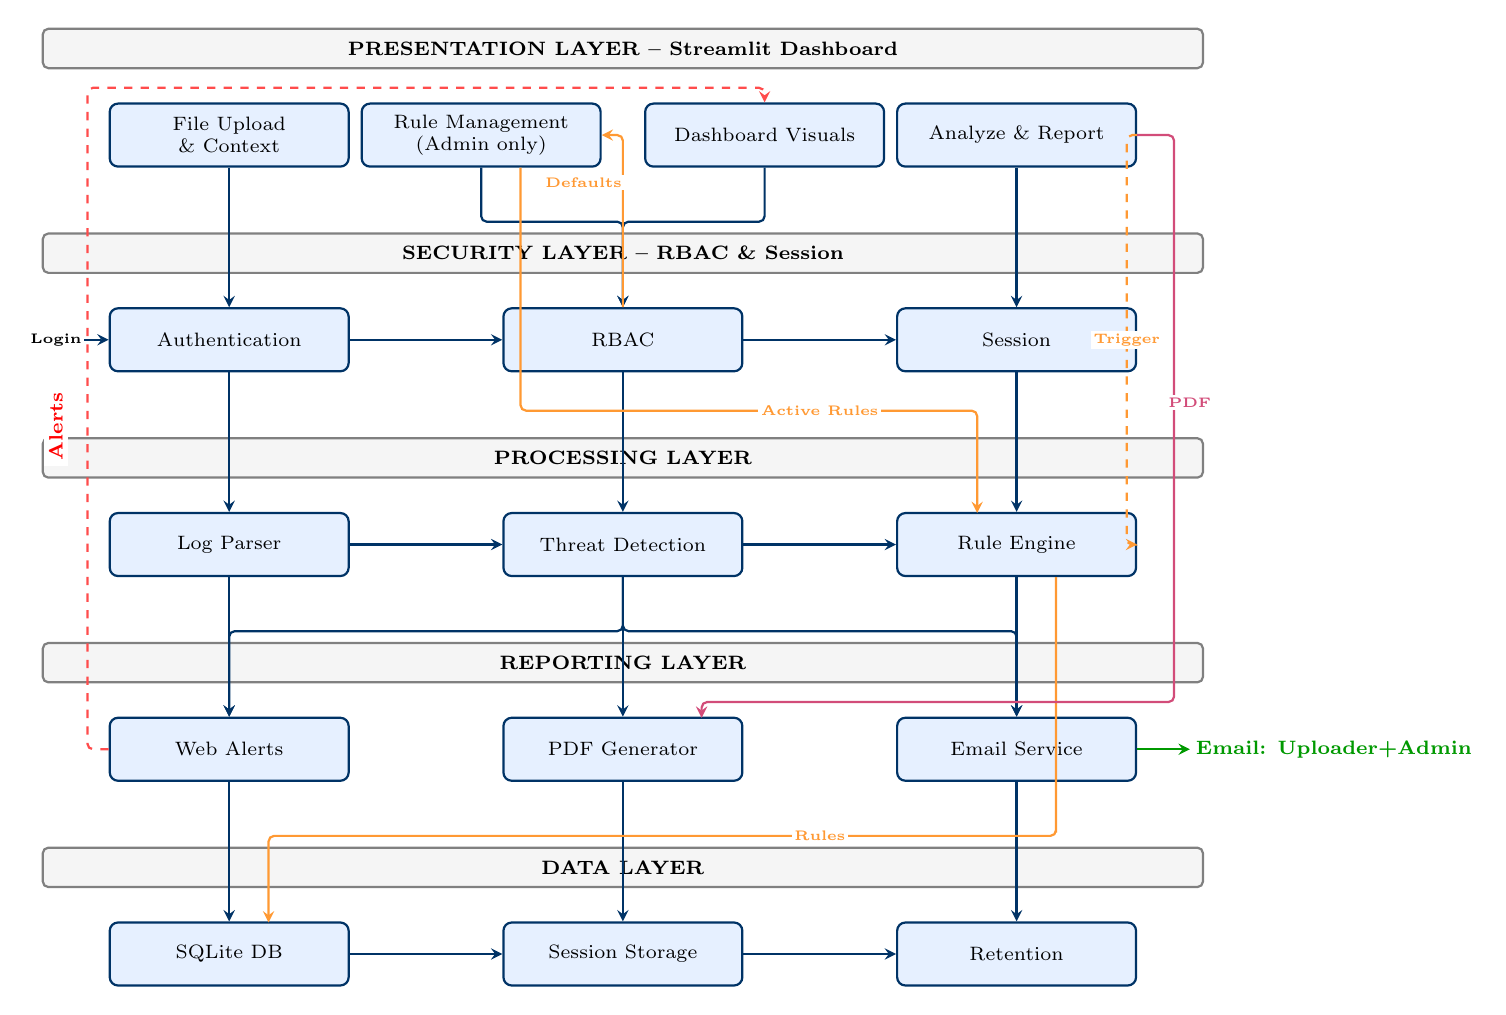
\begin{tikzpicture}[
    block/.style={
        rectangle,
        draw=darkblue,
        thick,
        fill=lightblue,
        text width=2.8cm,
        text centered,
        minimum height=0.8cm,
        font=\scriptsize,
        rounded corners=3pt,
        align=center
    },
    layer/.style={
        rectangle,
        draw=gray,
        thick,
        fill=lightgray,
        text width=14.5cm,
        text centered,
        minimum height=0.5cm,
        font=\bfseries\scriptsize,
        rounded corners=2pt
    },
    arrow/.style={thick, ->, >=stealth, draw=darkblue, rounded corners=2pt},
    alertarrow/.style={thick, ->, >=stealth, draw=red!70, dashed, rounded corners=2pt},
    emailarrow/.style={thick, ->, >=stealth, draw=green!60!black, rounded corners=2pt},
    reportarrow/.style={thick, ->, >=stealth, draw=purple!70, rounded corners=2pt},
    rulearrow/.style={thick, ->, >=stealth, draw=orange!80, rounded corners=2pt}
]

% ================= LAYERS =================
\node[layer] (l1) at (0,0) {PRESENTATION LAYER -- Streamlit Dashboard};
\node[layer] (l2) at (0,-2.6) {SECURITY LAYER -- RBAC \& Session};
\node[layer] (l3) at (0,-5.2) {PROCESSING LAYER};
\node[layer] (l4) at (0,-7.8) {REPORTING LAYER};
\node[layer] (l5) at (0,-10.4) {DATA LAYER};

% ================= BLOCKS =================
% Layer 1 Blocks
\node[block] (upload) at (-5.0,-1.1) {File Upload \& Context};
\node[block] (rulesel) at (-1.8,-1.1) {Rule Management\\(Admin only)};
\node[block] (dashboard) at (1.8,-1.1) {Dashboard Visuals};
\node[block] (buttons) at (5.0,-1.1) {Analyze \& Report};

% Layer 2 Blocks
\node[block] (auth) at (-5.0,-3.7) {Authentication};
\node[block] (rbac) at (0,-3.7) {RBAC};
\node[block] (session) at (5.0,-3.7) {Session};

% Layer 3 Blocks
\node[block] (parser) at (-5.0,-6.3) {Log Parser};
\node[block] (detection) at (0,-6.3) {Threat Detection};
\node[block] (rulesengine) at (5.0,-6.3) {Rule Engine};

% Layer 4 Blocks
\node[block] (webalert) at (-5.0,-8.9) {Web Alerts};
\node[block] (pdfgen) at (0,-8.9) {PDF Generator};
\node[block] (email) at (5.0,-8.9) {Email Service};

% Layer 5 Blocks
\node[block] (db) at (-5.0,-11.5) {SQLite DB};
\node[block] (sessiondata) at (0,-11.5) {Session Storage};
\node[block] (retention) at (5.0,-11.5) {Retention};

% ================= VERTICAL ARROWS =================
\draw[arrow] (upload.south) -- (auth.north);
\draw[arrow] (auth.south) -- (parser.north);
\draw[arrow] (parser.south) -- (webalert.north);
\draw[arrow] (webalert.south) -- (db.north);

\draw[arrow] (rbac.south) -- (detection.north);
\draw[arrow] (detection.south) -- (pdfgen.north);
\draw[arrow] (pdfgen.south) -- (sessiondata.north);

\draw[arrow] (session.south) -- (rulesengine.north);
\draw[arrow] (rulesengine.south) -- (email.north);
\draw[arrow] (email.south) -- (retention.north);

% Cross-column vertical inputs
\draw[arrow] (rulesel.south) -- (-1.8,-2.2) -- (0,-2.2) -- (rbac.north);
\draw[arrow] (dashboard.south) -- (1.8,-2.2) -- (0,-2.2) -- (rbac.north);
\draw[arrow] (buttons.south) -- (session.north);

% Cross-column processing outputs
\draw[arrow] (detection.south) -- (0,-7.4) -- (-5.0,-7.4) -- (webalert.north);
\draw[arrow] (detection.south) -- (0,-7.4) -- (5.0,-7.4) -- (email.north);

% ================= HORIZONTAL ARROWS =================
\draw[arrow] (auth.east) -- (rbac.west);
\draw[arrow] (rbac.east) -- (session.west);
\draw[arrow] (parser.east) -- (detection.west);
\draw[arrow] (detection.east) -- (rulesengine.west);
\draw[arrow] (db.east) -- (sessiondata.west);
\draw[arrow] (sessiondata.east) -- (retention.west);

% ================= RULE MANAGEMENT ARROWS (Orange) =================
% rulesel -> rulesengine (Active Rules)
\draw[rulearrow] (rulesel.south) ++(0.5,0) |- (4.5,-4.6) -- (4.5,-5.9);
\node[font=\tiny\bfseries\color{orange!80}, fill=white, inner sep=1pt] at (2.5,-4.6) {Active Rules};

% rulesengine -> db (Rules storage)
\draw[rulearrow] (rulesengine.south) ++(0.5,0) |- (5.5, -10.0) -- (-4.5, -10.0) -- (-4.5, -11.1);
\node[font=\tiny\bfseries\color{orange!80}, fill=white, inner sep=1pt] at (2.5,-10.0) {Rules};

% rbac -> rulesel (Defaults)
\draw[rulearrow] (rbac.north) |- (rulesel.east);
\node[font=\tiny\bfseries\color{orange!80}, fill=white, inner sep=1pt] at (-0.5,-1.7) {Defaults};

% buttons -> rulesengine (Trigger)
\draw[arrow, draw=orange!80, dashed] (buttons.east) -- (6.4, -1.1) |- (rulesengine.east);
\node[font=\tiny\bfseries\color{orange!80}, fill=white, inner sep=1pt] at (6.4,-3.7) {Trigger};

% ================= REPORTING ARROWS =================
% Web Alert Feedback (Red) - Fixed arrow path
\draw[alertarrow] (webalert.west) -- (-6.8, -8.9) -- (-6.8, -0.5) -| (dashboard.north);
\node[font=\scriptsize\bfseries\color{red}, fill=white, inner sep=2pt] at (-7.2,-4.8) [rotate=90] {Alerts};

% PDF Download (Purple) - Fixed arrow path
\draw[reportarrow] (buttons.east) -- (7.0, -1.1) |- (1.0, -8.3) -- (1.0, -8.5);
\node[font=\tiny\bfseries\color{purple!70}, fill=white, inner sep=1pt] at (7.2,-4.5) {PDF};

% Email to Uploader (+Admin) (Green)
\draw[emailarrow] (email.east) -- (7.2, -8.9);
\node[font=\scriptsize\bfseries\color{green!60!black}, fill=white, inner sep=2pt, anchor=west] at (7.2, -8.9) {Email: Uploader+Admin};

% ================= LOGIN FLOW (Fixed) =================
% Login arrow going INTO Authentication block
\draw[arrow] (-7.0, -3.7) -- (auth.west);
\node[font=\tiny\bfseries, fill=white, inner sep=1pt] at (-7.2, -3.7) {Login};

\end{tikzpicture}
\label{fig:architecture}
\end{figure}

\begin{table}[H]
\centering
\begin{tabular}{|p{3.5cm}|p{11cm}|}
\hline
\textbf{Layer} & \textbf{Components \& Responsibilities} \\
\hline
Presentation Layer & Streamlit dashboard with visualizations, multi-file upload, \textbf{Application / LeanIX context capture (IT Owner)}, registration interface, \textbf{Admin rule management UI}, \textbf{IT Owner read-only rule viewer} \\
\hline
Security Layer (RBAC) & Two-role access control (Administrator and IT Owner), Argon2id authentication, session management (15 min timeout), \textbf{Administrator-only rule modification}, \textbf{IT Owner read-only rule access} \\
\hline
Processing Layer & Multi-format log parsing, \textbf{Admin-configured rule engine}, vectorized threat detection, multi-file aggregation, executed in \textbf{process-isolated workers} for concurrency \\
\hline
Reporting Layer & Web UI alerts, PDF report generation (local download), SMTP email service \textbf{(uploader; plus the Administrator when an IT Owner runs it)} including the Application / LeanIX context \\
\hline
Data Layer & SQLite database (audit logs + \textbf{Admin-defined rules}), session-based temporary storage, retention policy (180 days for audit logs) \\
\hline
\end{tabular}
\label{tab:layers}
\end{table}

\newpage
\subsection{Complete System Workflow}

\begin{figure}[H]
\centering
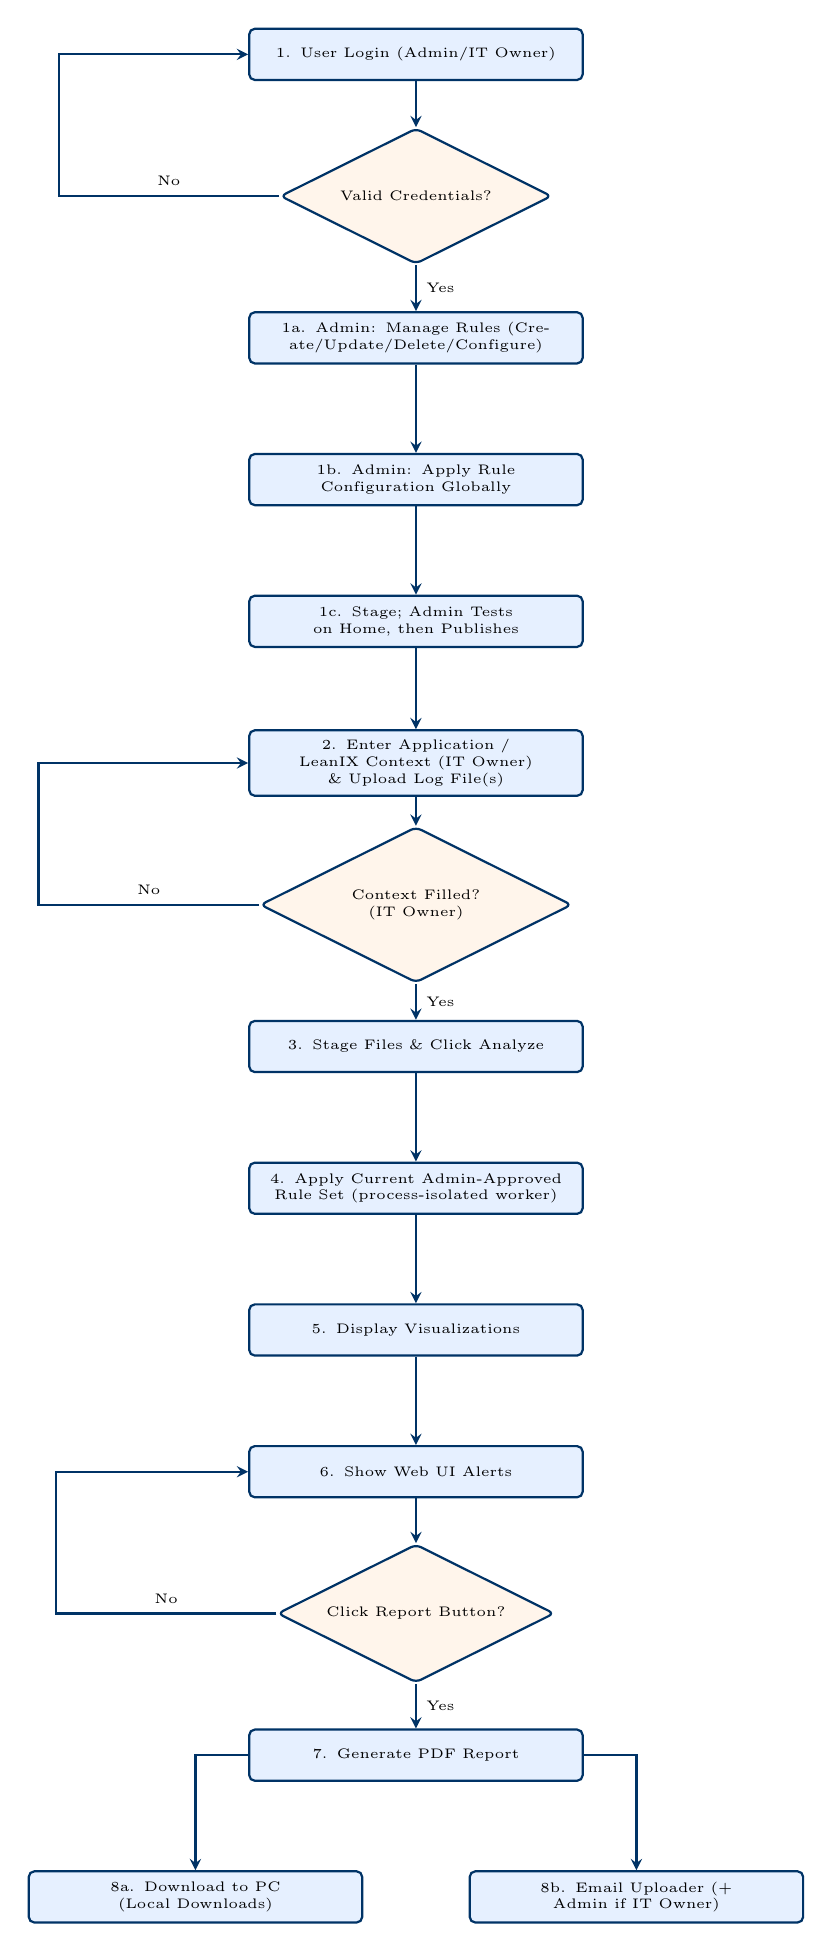
\begin{tikzpicture}[
    proc/.style={
        rectangle,
        draw=darkblue,
        thick,
        fill=lightblue,
        text width=4cm,
        text centered,
        minimum height=0.65cm,
        font=\tiny,
        rounded corners=2pt,
        align=center
    },
    decision/.style={
        diamond,
        draw=darkblue,
        thick,
        fill=lightorange,
        text width=2.5cm,
        text centered,
        minimum height=0.65cm,
        font=\tiny,
        rounded corners=2pt,
        aspect=2
    },
    arrow/.style={thick, ->, >=stealth, draw=darkblue}
]

% Vertical spacing increased to 1.8cm per step to perfectly cover the A4 text block height
\node[proc] (s1) at (0,0) {1. User Login (Admin/IT Owner)};
\node[decision] (s2) at (0,-1.8) {Valid Credentials?};
\node[proc] (s2a) at (0,-3.6) {1a. Admin: Manage Rules (Create/Update/Delete/Configure)};
\node[proc] (s2b) at (0,-5.4) {1b. Admin: Apply Rule Configuration Globally};
\node[proc] (s2c) at (0,-7.2) {1c. Stage; Admin Tests on Home, then Publishes};
\node[proc] (s3) at (0,-9.0) {2. Enter Application / LeanIX Context (IT Owner) \& Upload Log File(s)};
\node[decision] (s4) at (0,-10.8) {Context Filled? (IT Owner)};
\node[proc] (s6) at (0,-12.6) {3. Stage Files \& Click Analyze};

\node[proc] (s7) at (0,-14.4) {4. Apply Current Admin-Approved Rule Set (process-isolated worker)};
\node[proc] (s8) at (0,-16.2) {5. Display Visualizations};
\node[proc] (s9) at (0,-18.0) {6. Show Web UI Alerts};
\node[decision] (s10) at (0,-19.8) {Click Report Button?};
\node[proc] (s11) at (0,-21.6) {7. Generate PDF Report};

% Parallel branches for Download and Email
\node[proc] (s12) at (-2.8,-23.4) {8a. Download to PC (Local Downloads)};
\node[proc] (s13) at (2.8,-23.4) {8b. Email Uploader (+ Admin if IT Owner)};

% Draw main vertical and loopback arrows
\draw[arrow] (s1) -- (s2);
\draw[arrow] (s2) -- node[right, font=\tiny] {Yes} (s2a);
\draw[arrow] (s2.west) -- node[above, font=\tiny] {No} ++(-2.8,0) |- (s1.west);
\draw[arrow] (s2a) -- (s2b);
\draw[arrow] (s2b) -- (s2c);
\draw[arrow] (s2c) -- (s3);
\draw[arrow] (s3) -- (s4);

% Context gate: an IT Owner must supply Application/LeanIX before analysis can start
\draw[arrow] (s4) -- node[right, font=\tiny] {Yes} (s6);
\draw[arrow] (s4.west) -- node[above, font=\tiny] {No} ++(-2.8,0) |- (s3.west);
\draw[arrow] (s6) -- (s7);

% Continue main flow
\draw[arrow] (s7) -- (s8);
\draw[arrow] (s8) -- (s9);
\draw[arrow] (s9) -- (s10);
\draw[arrow] (s10) -- node[right, font=\tiny] {Yes} (s11);
\draw[arrow] (s10.west) -- node[above, font=\tiny] {No} ++(-2.8,0) |- (s9.west);

% Draw branching arrows for final report generation
\draw[arrow] (s11.west) -| (s12.north);
\draw[arrow] (s11.east) -| (s13.north);

\end{tikzpicture}
\caption{Complete System Workflow}
\label{fig:workflow}
\end{figure}

\subsection{Supported Log File Formats}

The system supports secure upload and analysis of multiple industry-standard log file formats:

\begin{table}[H]
\centering
\begin{tabular}{|l|l|l|}
\hline
\textbf{Format} & \textbf{Extension} & \textbf{Description} \\
\hline
Raw Text Log & .log, .txt & Generic server and application logs \\
\hline
Syslog & .syslog & Standard Linux/Unix system logs \\
\hline
CEF Format & .cef & Common Event Format (SIEM compatible) \\
\hline
Web Server Logs & .log & Apache/Nginx access and error logs \\
\hline
\end{tabular}
\label{tab:formats}
\end{table}

\subsection{Dashboard Visualizations}

The Streamlit dashboard presents the following visualizations and analysis tools after log analysis:

\begin{table}[H]
\centering
\begin{tabular}{|p{4cm}|p{10cm}|}
\hline
\textbf{Visualization / Tool} & \textbf{Description} \\
\hline
Threat Summary Cards & Display counts of CRITICAL, HIGH, MEDIUM, LOW threats with color-coded backgrounds \\
\hline
Severity Distribution Chart & Pie chart showing percentage distribution of threat severities \\
\hline
Threat Timeline Graph & Line chart showing threat frequency over time \\
\hline
Top Attack Sources & Bar chart of IP addresses with most threat occurrences \\
\hline
Top Involved Users & Bar chart of usernames most frequently involved in findings \\
\hline
Threat Type Distribution & Horizontal bar chart of different threat types detected \\
\hline
Findings by Rule Type & Static vs behavioral finding counts \\
\hline
Threats by Rule (Table) & Aggregated count of findings per rule \\
\hline
Detailed Threat Table & Sortable table with timestamp, severity, type, description, source IP \\
\hline
Findings Search & Free-text search across findings (IP, username, rule, description) \\
\hline
Findings CSV Export & Download the complete findings table as CSV (full, untruncated data) \\
\hline
Files Analyzed List & Lists every log file included in the current analysis run \\
\hline
\textbf{Admin Rule Management Panel} & Admin-only interface for creating, modifying, deleting detection rules \\
\hline
\textbf{IT Owner Rule Viewer} & Read-only, severity-ordered (Critical $\rightarrow$ Low), colour-coded cards showing every active rule's detection logic, severity, threshold, time window, group-by key, recommended action and framework mapping (MITRE / OWASP / NIST / ISO 27001 / CERT-In), plus the active rule-set version stamp \\
\hline
\end{tabular}
\caption{Dashboard Visualization Components}
\label{tab:visualizations}
\end{table}

\subsection{Concurrency and Scalability}

To remain responsive when many IT Owners use the system simultaneously, the heavy
log analysis (parsing + rule evaluation) does \textbf{not} run inside the web-server
process. Instead:

\begin{itemize}
    \item Each analysis job is executed in a \textbf{separate, process-isolated worker}
          so CPU-bound work never blocks the
          Streamlit server's interpreter (avoids the Python GIL bottleneck).
    \item A \textbf{bounded worker pool} (\texttt{services/analysis\_runner.py}) caps how
          many analyses run concurrently so a burst of users cannot exhaust CPU/RAM;
          additional jobs queue until a worker frees up.
    \item If a worker process cannot be launched, the system \textbf{falls back to
          in-process analysis} automatically, so functionality is never lost.
    \item A worker crash is \textbf{isolated} and cannot bring down the web server.
\end{itemize}

\subsection{Database Schema}

The SQLite database shall consist of the following tables:

\begin{longtable}{|p{4.2cm}|p{11cm}|}
\hline
\textbf{Table Name} & \textbf{Purpose and Columns} \\
\hline
users & User credentials (username, password\_hash, email, role, created\_at, password\_changed\_at, password\_expiry, last\_login, is\_active, password\_type, is\_first\_login) \\
\hline
audit\_logs & User action trail (user\_id, action, timestamp, ip\_address, details, file\_name, \textbf{application}, \textbf{leanix\_id}) \\
\hline
sessions & Active sessions (user\_id, session\_token, created\_at, last\_activity, expiry\_time) \\
\hline
password\_history & Password change history (user\_id, password\_hash, created\_at) \\
\hline
\textbf{pending\_registrations} & \textbf{Unactivated IT Owner sign-ups (id, username, email, temp\_password\_hash, created\_at); a row is promoted to a \texttt{users} record once the registrant sets a permanent password, then deleted. Auto-expires after 7 days.} \\
\hline
\textbf{detection\_rules} & \textbf{Built-in and admin/custom rules (id, rule\_name,
rule\_type [static\,$\vert$\,behavioral\,$\vert$\,custom], condition, severity, description,
is\_static, default\_threshold, time\_window\_seconds, group\_by, is\_enabled,
detection\_logic, recommended\_action, framework\_refs, example\_log, why\_suspicious,
security\_impact, is\_propagated [published flag], created\_by, created\_at, updated\_at)} \\
\hline
\caption{Database Schema}
\label{tab:schema}
\end{longtable}



\subsection{Password-Related Database Fields}

\begin{table}[H]
\centering
\begin{tabular}{|p{4cm}|p{10cm}|}
\hline
\textbf{Column Name} & \textbf{Purpose} \\
\hline
password\_hash & Argon2id hash (temporary or permanent) \\
\hline
password\_type & ENUM('temporary', 'permanent') \\
\hline
password\_changed\_at & Timestamp of password creation \\
\hline
password\_expiry & Expiry timestamp for permanent passwords (180 days) \\
\hline
is\_first\_login & Flag for forcing password change \\
\hline
\end{tabular}
\caption{Password-Related Database Fields}
\label{tab:password-fields}
\end{table}

\subsection{Password State Management}

\begin{table}[H]
\centering
\begin{tabular}{|p{3cm}|p{4cm}|p{7cm}|}
\hline
\textbf{State} & \textbf{Duration} & \textbf{Description} \\
\hline
Temporary & First login only & Generated during registration, sent via email, forces change on first login \\
\hline
Active & Days 1-179 & Permanent password valid, normal access \\
\hline
Expired & Day 180+ & Forces password change at next login with popup notification \\
\hline
\end{tabular}
\caption{IT Owner Password States}
\label{tab:password-states}
\end{table}


\section{Threat Detection Rules}

The system ships with a curated library of \textbf{45 detection rules} organized into two
categories. Every rule is mapped to recognized security frameworks
(\textbf{MITRE ATT\&CK}, \textbf{OWASP Top 10 / API}, \textbf{NIST SP 800-53},
\textbf{ISO/IEC 27001 Annex A} and \textbf{CERT-In}), and each carries presentation
metadata --- plain-language \emph{detection logic}, a concise \emph{recommended action},
\emph{framework references} and an \emph{example log line} --- so the dashboard can render a
full, data-driven card for every rule. \textbf{IT Owners can view all active rules}
(including thresholds, time windows and framework mappings) through the read-only rule viewer.

\begin{table}[H]
\centering
\begin{tabular}{|p{3.4cm}|p{11.1cm}|}
\hline
\textbf{Category} & \textbf{Description} \\
\hline
Static (Signature) Rules & Fixed regular-expression / signature conditions (SQL injection, XSS, path traversal, web shells, reverse shells, etc.). Fire on a single matching log line. \\
\hline
Behavioral (Threshold) Rules & Count events grouped by Source IP / Username / Whole-file and fire when a configurable count is met within a time window (brute force, credential stuffing, error spikes, etc.). Admin no-code rules are behavioral rules authored from the Web UI (pattern + threshold + time window + group-by), with no Python changes. \\
\hline
\end{tabular}
\label{tab:rule-categories}
\end{table}
\subsection{User Behavior Analysis Rules (Static)}

\begin{table}[H]
\centering
\begin{tabular}{|p{4.2cm}|p{1.7cm}|p{4.6cm}|p{4.2cm}|}
\hline
\textbf{Rule Name} & \textbf{Severity} & \textbf{What It Detects} & \textbf{Frameworks} \\
\hline
Dormant Account Activity & HIGH & Long-inactive account suddenly becomes active & MITRE T1078; NIST AC-2(3) \\
\hline
Concurrent Sessions & HIGH & One account with simultaneous sessions from different sources & MITRE T1078; NIST AC-10 \\
\hline
Geographic Anomaly & MEDIUM & Login from an unusual region / impossible travel & MITRE T1078; NIST AC-7 \\
\hline
Unusual Working Hours & LOW & Majority of activity outside 09:00--17:00 & MITRE T1078; NIST AU-6 \\
\hline
Off-Hours Access & MEDIUM & Successful login between 00:00 and 05:00 & MITRE T1078; NIST AU-6 \\
\hline
\end{tabular}
\caption{User Behavior Analysis Rules (Static)}
\label{tab:user-behavior-rules}
\end{table}

\subsection{Static Attack-Pattern Detection Rules}

\begin{longtable}{|p{4.2cm}|p{1.7cm}|p{4.6cm}|p{4.2cm}|}
\hline
\textbf{Rule Name} & \textbf{Severity} & \textbf{What It Detects} & \textbf{Frameworks} \\
\hline
\endfirsthead
\hline
\textbf{Rule Name} & \textbf{Severity} & \textbf{What It Detects} & \textbf{Frameworks} \\
\hline
\endhead
\hline
\multicolumn{4}{|r|}{\textit{Continued on next page}} \\
\hline
\endfoot
\hline
\endlastfoot
SQL Injection Attempt & HIGH & UNION SELECT, OR 1=1, DROP TABLE, stored-procedure abuse & MITRE T1190; OWASP A03; NIST SI-10 \\
\hline
Path Traversal Attempt & HIGH & ../ and URL-encoded variants escaping the web root & MITRE T1083; OWASP A01; NIST AC-3 \\
\hline
Command Injection & CRITICAL & Shell metacharacters (; | \&\& \$() ``) chained with OS commands & MITRE T1059; OWASP A03; NIST SI-10 \\
\hline
XSS Attempt & MEDIUM & Script tags, JS event handlers, javascript:/vbscript: URIs & MITRE T1059.007; OWASP A03; NIST SI-10 \\
\hline
Directory Scanning & MEDIUM & Probing of admin panels, .git/.env, config/backup files & MITRE T1595.003; OWASP A05; NIST RA-5 \\
\hline
Abnormal HTTP Methods & HIGH & TRACE, CONNECT and WebDAV verbs used in recon & MITRE T1595; OWASP A05; NIST CM-7 \\
\hline
\end{longtable}



\subsection{Access Control Detection Rules (Static)}

\begin{table}[H]
\centering
\begin{tabular}{|p{4.2cm}|p{1.9cm}|p{4.6cm}|p{4.2cm}|}
\hline
\textbf{Rule Name} & \textbf{Severity} & \textbf{What It Detects} & \textbf{Frameworks} \\
\hline
Unauthorized Access Attempt & HIGH & HTTP 401/403 and access-denied responses & MITRE T1190; OWASP A01; NIST AC-3 \\
\hline
Privilege Escalation & CRITICAL & sudo/su abuse, role grants, SUID, gained root/admin & MITRE T1068/T1548; NIST AC-6 \\
\hline
Sensitive Resource Access & HIGH & /etc/passwd, /etc/shadow, SSH keys, *.pem, secret stores & MITRE T1552; NIST AC-3 \\
\hline
API Key Misuse & MEDIUM & Invalid/expired/revoked API keys and bearer tokens & MITRE T1552.001; OWASP API2; NIST IA-5 \\
\hline
Session Hijacking Pattern & CRITICAL & Session fixation/hijacking, token mismatch, CSRF & MITRE T1539; OWASP A07; NIST SC-23 \\
\hline
Account Lockout Event & HIGH & Account locked after exceeding failed-auth threshold & MITRE T1110; NIST AC-7 \\
\hline
Successful Login After Failures & MEDIUM & Login success right after 3+ consecutive failures & MITRE T1110; NIST AC-7 \\
\hline
\end{tabular}
\caption{Access Control Detection Rules (Static)}
\label{tab:access-rules}
\end{table}
\newpage
\subsection{Modern / Advanced Threat Coverage (Static)}

These rules extend the library with current attacker techniques and notable CVEs, each mapped
to MITRE ATT\&CK.

\begin{longtable}{|p{4.2cm}|p{1.9cm}|p{4.6cm}|p{4.2cm}|}
\hline
\textbf{Rule Name} & \textbf{Severity} & \textbf{What It Detects} & \textbf{Frameworks} \\
\hline
\endfirsthead
\hline
\textbf{Rule Name} & \textbf{Severity} & \textbf{What It Detects} & \textbf{Frameworks} \\
\hline
\endhead
\hline
\multicolumn{4}{|r|}{\textit{Continued on next page}} \\
\hline
\endfoot
\hline
\endlastfoot
Log4Shell / JNDI Injection & CRITICAL & jndi:ldap/rmi/dns lookup payloads (CVE-2021-44228) & MITRE T1190; CVE-2021-44228; CERT-In \\
\hline
Web Shell Upload / Access & CRITICAL & Known shell names, eval-over-base64, scripts in upload paths & MITRE T1505.003; OWASP A03; NIST SI-3 \\
\hline
PowerShell Encoded Command & HIGH & Encoded/hidden PowerShell, IEX / DownloadString & MITRE T1059.001; NIST SI-4 \\
\hline
Credential Dumping & CRITICAL & LSASS dumps, NTDS.dit / SAM extraction, known tools & MITRE T1003; NIST IR-4 \\
\hline
Reverse Shell Indicator & CRITICAL & bash to /dev/tcp, nc -e, mkfifo|nc, python socket shells & MITRE T1059/T1571; NIST SC-7 \\
\hline
DNS Tunneling / Exfiltration & HIGH & Long high-entropy subdomains, TXT abuse, known tooling & MITRE T1048.003/T1071.004; NIST SC-7 \\
\hline
Cloud Metadata SSRF & HIGH & Requests to 169.254.169.254 / cloud IMDS endpoints & MITRE T1552.005; OWASP A10; NIST SC-7 \\
\hline
Ransomware File Activity & CRITICAL & Mass-rename to crypto extensions, ransom-note creation & MITRE T1486; NIST CP-9 \\
\hline
XML External Entity (XXE) & HIGH & External ENTITY/DOCTYPE, file:// / php://filter wrappers & MITRE T1190; OWASP A05; NIST SI-10 \\
\hline
LDAP Injection & HIGH & LDAP filter metacharacters (*), )(, (| in directory queries & MITRE T1190; OWASP A03; NIST SI-10 \\
\hline
Server-Side Request Forgery (SSRF) & HIGH & User URL targeting loopback / RFC1918 internal ranges & MITRE T1090; OWASP A10; NIST SC-7 \\
\hline
Security Scanner Activity & MEDIUM & sqlmap, nikto, nmap, nuclei and similar tool signatures & MITRE T1595; OWASP A05; NIST RA-5 \\
\hline
OAuth / Token Abuse & MEDIUM & Refresh-token reuse/revocation, bad redirect\_uri, consent phishing & MITRE T1528; NIST IA-5 \\
\hline
\end{longtable}
\newpage
\subsection{Behavioral Detection Rules (Configurable Thresholds)}

Behavioral rules aggregate events by the listed \textbf{Group-by} key and fire when the
\textbf{Default} count is met within the time window. All defaults follow industry guidance
(NIST SP 800-63B, OWASP ASVS) and are fully Administrator-configurable from the Web UI.

\begin{longtable}{|p{3.7cm}|p{3.0cm}|p{2.1cm}|p{1.9cm}|p{3.0cm}|}
\hline
\textbf{Rule Name} & \textbf{Default} & \textbf{Group-by} & \textbf{Severity} & \textbf{Frameworks} \\
\hline
\endfirsthead
\hline
\textbf{Rule Name} & \textbf{Default} & \textbf{Group-by} & \textbf{Severity} & \textbf{Frameworks} \\
\hline
\endhead
\hline
\multicolumn{5}{|r|}{\textit{Continued on next page}} \\
\hline
\endfoot
\hline
\endlastfoot
Brute Force Attack & $\geq 5$ in 60 sec & Source IP & CRITICAL & MITRE T1110.001; NIST AC-7 \\
\hline
Repeated Failed Logins & $\geq 5$ in 15 min & Username & HIGH & MITRE T1110; NIST AC-7 \\
\hline
Rapid Login Attempts & $\geq 20$ in 10 sec & Whole file & CRITICAL & MITRE T1110.004; NIST AC-7 \\
\hline
Multiple User Failures & $\geq 5$ users in 5 min & Source IP & HIGH & MITRE T1110.004; NIST AC-7 \\
\hline
Repeated Access Denials & $\geq 10$ in 5 min & Source IP & HIGH & MITRE T1190; NIST AC-3 \\
\hline
Error Rate Spike & $\geq 50$ in 5 min & Whole file & MEDIUM & MITRE T1499; NIST SI-4 \\
\hline
Service Crash Loop & $\geq 3$ in 2 min & Whole file & HIGH & MITRE T1499; NIST SI-4 \\
\hline
Rapid Sequential Actions & $\geq 50$ in 60 sec & Whole file & MEDIUM & MITRE T1499; NIST SI-4 \\
\hline
Mass Data Access & $\geq 1000$ in 1 hr & Whole file & MEDIUM & MITRE T1530/T1213; NIST AC-6 \\
\hline
Resource Exhaustion & Any occurrence & Whole file & HIGH & MITRE T1499.001; NIST SC-5 \\
\hline
Unexpected Shutdown & Any occurrence & Whole file & HIGH & MITRE T1529; NIST IR-4 \\
\hline
Configuration Change & Any occurrence & Whole file & MEDIUM & MITRE T1562; NIST CM-3 \\
\hline
Database Error Spike & $\geq 20$ in 5 min & Whole file & MEDIUM & MITRE T1190; NIST SI-4 \\
\hline
\end{longtable}

\subsection{No-Code Behavioral Rules (Admin-Authored)}

Administrators can build entirely new detection logic from the dashboard --- no Python
required --- by supplying a keyword/regex \textbf{pattern}, a \textbf{threshold}, a
\textbf{time window} and a \textbf{group-by} key (Source IP / Username / Whole file). These
no-code rules are \textbf{behavioral} rules: they are evaluated by the same vectorized engine
as the built-in rules and appear in results and the PDF report with their concise recommended
action. A reference example ships by default:

\begin{table}[H]
\centering
\begin{tabular}{|p{3.7cm}|p{3.0cm}|p{2.1cm}|p{1.7cm}|p{3.0cm}|}
\hline
\textbf{Rule Name} & \textbf{Default} & \textbf{Group-by} & \textbf{Severity} & \textbf{Frameworks} \\
\hline
MFA Fatigue / Push Bombing & $\geq 5$ in 5 min & Username & HIGH & MITRE T1621; NIST IA-2 \\
\hline
\end{tabular}
\caption{No-Code Behavioral Rule (shipped example)}
\label{tab:custom-rules}
\end{table}

\subsection{Framework Alignment and Rule Metadata}

Every rule record stores framework references and presentation metadata, making the rule
viewer fully data-driven (including for admin-authored no-code rules):

\begin{table}[H]
\centering
\begin{tabular}{|p{4cm}|p{10cm}|}
\hline
\textbf{Metadata Field} & \textbf{Purpose} \\
\hline
detection\_logic & Plain-language description of how and when the rule fires \\
\hline
recommended\_action & Concise ($\leq 2$ line) mitigation / investigation step shown on the card and PDF \\
\hline
framework\_refs & MITRE ATT\&CK / OWASP / NIST 800-53 / ISO 27001 / CERT-In mapping \\
\hline
example\_log & A representative log line that would trigger the rule \\
\hline
group\_by & Aggregation key for threshold rules (source\_ip / username / global) \\
\hline
\end{tabular}
\caption{Rule Presentation and Framework Metadata}
\label{tab:rule-metadata}
\end{table}


\section{Software Bill of Materials (SBOM)}

\begin{longtable}{|p{3.5cm}|p{1.5cm}|p{6cm}|p{5cm}|}
\hline
\textbf{Component} & \textbf{Version} & \textbf{Vendor} & \textbf{Tag} \\
\hline
\endfirsthead
\hline
\textbf{Component} & \textbf{Version} & \textbf{Vendor} & \textbf{Tag} \\
\hline
\endhead
\hline
\multicolumn{4}{|r|}{\textit{Continued on next page}} \\
\hline
\endfoot
\hline
\endlastfoot

Visual Studio Code & 1.122.0 & Microsoft Corporation & Code Editor / IDE \\
Anaconda (Conda) & 25.3.0 & Anaconda, Inc. & Python Distribution \\
Python & 3.12.13 & Python Software Foundation & Programming Language \\
Streamlit & 1.54.0 & Streamlit Inc. & Web Dashboard \\
SQLAlchemy & 2.0.41 & SQLAlchemy Authors & ORM / Database \\
Pandas & 2.2.3 & Pandas Development Team & Data Processing \\
Plotly & 6.5.0 & Plotly Technologies Inc. & Visualization \\
ReportLab & 4.3.1 & ReportLab Inc. & PDF Generation \\
PyYAML & 6.0.2 & PyYAML Contributors & Configuration \\
Cryptography & 48.0.1 & PyCA & Encryption / Security \\
Passlib & 1.7.4 & Passlib Project & Password Hashing \\
argon2-cffi & 23.1.0 & argon2-cffi Contributors & Password Hashing \\
bcrypt & 4.3.0 & OpenBSD Project & Password Hashing \\
python-dotenv & 1.2.2 & Dotenv Project & Secret Management \\
email-validator & 2.3.0 & email-validator Contributors & Email Validation \\
itsdangerous & 2.2.0 & Pallets Projects & Session Security \\
watchdog & 6.0.0 & Watchdog Project & File Monitoring \\
tzdata & 2026.2 & Python Software Foundation (IANA) & Timezone Database (IST on Windows) \\
pytest & 9.0.3 & Pytest Project & Testing \\
pytest-cov & 6.1.1 & pytest-cov Contributors & Test Coverage \\
bandit & 1.8.3 & Python Code Quality Authority & Static Application Security \\
pip-audit & 2.9.0 & Python Packaging Authority & Vulnerability Scanning \\
msgpack & 1.2.1 & MessagePack / Inada Naoki & Serialization (transitive via pip-audit; security-pinned) \\

\end{longtable}
\label{tab:sbom}

\newpage
\section{Email Report Sample}

When a report is generated, the user who uploaded the file receives an email with the PDF report and the findings CSV attached. \textbf{When an IT Owner generates the report, a copy is also sent to the Administrator (with the IT Owner's username prefixed to the subject); an Administrator's own report is sent to the Administrator only.} An IT Owner report carries the \textbf{Application / Product} and \textbf{LeanIX ID / PIF ID} in both the subject and the body; the Administrator's own report omits the Application, LeanIX and ``Rules Applied'' lines.

\begin{small}
\begin{verbatim}
Subject: AZURE | 2345-Log Analysis Report-Jun 20,2026
   (Admin copy when an IT Owner runs it -- username prefixed:
    "userx : AZURE | 2345-Log Analysis Report-Jun 20,2026")
   (Administrator's own report has no context:
    "Log Analysis Report-20 Jun,2026")

Dear userx,

The security analysis of the uploaded log file(s) has been completed.
A summary of the findings is provided below.

Report Details:
-----------------
Application/Product:   AZURE                 <- IT Owner reports only
LeanIX ID / PIF ID:    2345                  <- IT Owner reports only
Generated By:          userx (user@companyname.com)
Analysis Date:         20-06-2026 14:32:10 IST
Rules Applied:         Administrator-approved rule set    <- IT Owner reports only

Files Analyzed:
-----------------
1. server_log_jun18.log
2. server_log_jun19.log
3. server_log_jun20.log

Threat Summary:
-----------------
Total Threats:    23
Critical:         3
High:             8
Medium:           7
Low:              5

Attached:  security_report_20-06-2026.pdf
           threat_findings_20260620_143210.csv

For detailed results, please refer to the attached PDF report and the
complete findings table in CSV format.

Note: This report is NOT stored on the server. Please save a copy for your records.

Best Regards,
Cybersecurity Log Intelligence System
\end{verbatim}
\end{small}



\newpage
\section{Setup and Installation Guide}

\subsection{Project Directory Structure}

\noindent The project follows a modular architecture to improve maintainability, scalability, and separation of concerns. The directory structure is organized as follows:

\vspace{0.3cm}

\begin{tcolorbox}[colback=blue!3!white, colframe=darkblue, arc=5pt, boxrule=0.8pt, left=5pt, right=5pt, top=5pt, bottom=5pt, fontupper=\ttfamily\scriptsize]
\begin{verbatim}
Cybersecurity Log Intelligence System/
|
+-- main.py                         # Application entry point
+-- app.py                          # Streamlit routing
+-- .env                            # Environment secrets (copy from .env.example)
+-- .env.example                    # Environment template
+-- .gitignore                      # Files excluded from version control
+-- requirements.txt                # Python dependencies
+-- .bandit                         # Bandit scan config (excludes tests/ + Testcases/)
|
+-- .streamlit/
|   +-- config.toml                 # Streamlit theme + server config
|
+-- config/
|   +-- settings.py                 # App constants, IST timezone, worker settings
|   +-- detection_rules.yaml        # Default detection rules
|
+-- database/
|   +-- models.py                   # SQLAlchemy ORM models
|   +-- db.py                       # Database engine & session
|   +-- init_db.py                  # Tables + admin + rules setup
|
+-- auth/
|   +-- password.py                 # Argon2id hashing & policy
|   +-- session_manager.py          # Session CRUD & 15-min timeout
|   +-- access_control.py           # Role-based access guards
|
+-- services/
|   +-- audit_service.py            # Audit logging (IST timestamps)
|   +-- email_service.py            # SMTP email with PDF attachments
|   +-- user_service.py             # User CRUD & authentication
|   +-- log_parser.py               # Multi-format log parsing
|   +-- threat_engine.py            # Static & behavioral rule evaluation (vectorized)
|   +-- _static_match.py            # Stdlib-only regex matcher for spawned workers
|   +-- recommendations.py          # Remediation guidance
|   +-- report_service.py           # PDF generation (in-memory)
|   +-- analysis_runner.py          # Bounded-concurrency job submission
|   +-- analysis_worker.py          # Process-isolated analysis worker
|
+-- ui/
|   +-- components.py               # CSS, navigation, charts
|   +-- login_page.py               # Login + Forgot Password + Admin Setup
|   +-- register_page.py            # IT Owner registration
|   +-- dashboard_page.py           # Home: upload + analyze + results (all-in-one)
|   +-- rules_page.py               # Rule viewer (Admin + IT Owner)
|   +-- users_page.py               # User management (Admin only)
|   +-- settings_page.py            # SMTP config + Change Password
|   +-- audit_page.py               # Audit logs (Admin only)
|
+-- utils/
|   +-- validators.py               # Input validation
|   +-- temp_file_manager.py        # Auto-cleanup of temp files
|   +-- crypto_utils.py             # Cryptographic helpers
|
+-- tests/
|   +-- conftest.py                 # Test fixtures
|   +-- test_password.py            # Password policy tests
|   +-- test_log_parser.py          # Log parsing tests
|   +-- test_threat_engine.py       # Rule engine tests
|   +-- test_user_service.py        # User service tests
|
+-- Testcases/                      # Per-rule .log samples + security test scripts
|   +-- <Rule Name>.log             # One sample per detection rule
|   +-- fuzz_test.py                # Fuzz harness (parsers, extractors, rule engine)
|   +-- generate_all_threats_log.py # Log generator covering every rule
|
+-- temp/                           # Temporary uploaded files (auto-cleaned)
\end{verbatim}
\end{tcolorbox}



\subsection{Complete Installation Script}

\subsubsection{Step 1: Create Conda Environment}

\begin{tcolorbox}[colback=gray!10!white, colframe=gray!70!black, arc=3pt, boxrule=0.5pt]
\begin{verbatim}
conda create -n cybersec python=3.12 -y
\end{verbatim}
\end{tcolorbox}

\subsubsection{Step 2: Activate Environment}

\begin{tcolorbox}[colback=gray!10!white, colframe=gray!70!black, arc=3pt, boxrule=0.5pt]
\begin{verbatim}
conda activate cybersec
\end{verbatim}
\end{tcolorbox}

\subsubsection{Step 3: Upgrade pip}

\begin{tcolorbox}[colback=gray!10!white, colframe=gray!70!black, arc=3pt, boxrule=0.5pt]
\begin{verbatim}
python -m pip install --upgrade pip
\end{verbatim}
\end{tcolorbox}

\subsubsection{Step 4: Install Core Packages}

\begin{tcolorbox}[colback=gray!10!white, colframe=gray!70!black, arc=3pt, boxrule=0.5pt]
\begin{verbatim}
pip install streamlit==1.54.0 sqlalchemy==2.0.41 passlib==1.7.4 
argon2-cffi==23.1.0 pandas==2.2.3 plotly==6.5.0 reportlab==4.3.1 
pyyaml==6.0.2 email-validator==2.3.0 python-dotenv==1.2.2 
bcrypt==4.3.0 itsdangerous==2.2.0 cryptography==48.0.1
watchdog==6.0.0 tzdata==2026.2
\end{verbatim}
\end{tcolorbox}


\subsubsection{Step 5: Install Development and Security Tools}

\begin{tcolorbox}[colback=gray!10!white, colframe=gray!70!black, arc=3pt, boxrule=0.5pt]
\begin{verbatim}
pip install bandit==1.8.3 pip-audit==2.9.0
\end{verbatim}
\end{tcolorbox}

\subsubsection{Step 6: Install Testing Tools}

\begin{tcolorbox}[colback=gray!10!white, colframe=gray!70!black, arc=3pt, boxrule=0.5pt]
\begin{verbatim}
pip install pytest==9.0.3 pytest-cov==6.1.1
\end{verbatim}
\end{tcolorbox}

\begin{tcolorbox}[colback=green!5!white, colframe=green!60!black, arc=3pt, boxrule=0.5pt]
\textbf{Tip:} You can install everything in one step with
\texttt{pip install -r requirements.txt} instead of Steps 4--6.
\end{tcolorbox}

\subsubsection{Step 7: Configure Environment Variables}

\noindent Open the \texttt{.env} and configure the required values :

\begin{itemize}
    \item \textbf{Generate a secure APP\_SECRET\_KEY:} Run this command in your terminal:
\end{itemize}

\begin{tcolorbox}[colback=gray!10!white, colframe=gray!70!black, arc=3pt, boxrule=0.5pt]
\begin{verbatim}
python -c "import secrets; print(secrets.token_hex(32))"
\end{verbatim}
\end{tcolorbox}

\begin{itemize}
    \item \textbf{Set SMTP\_USER:} Enter your Gmail email address
    
    \item \textbf{Generate a 16-digit SMTP\_PASS (App Password):}
    \begin{enumerate}
        \item Verify that 2-Factor Authentication is enabled on your Gmail account
        \item Navigate to \url{https://myaccount.google.com/apppasswords}
        \item Enter a name for the app (e.g., "Cybersecurity Log System")
        \item Click "Generate" to create a 16-digit App Password
        \item Copy the generated password and paste it as \texttt{SMTP\_PASS} in your \texttt{.env} file
    \end{enumerate}

    \item \textbf{(Optional) Concurrency tuning:} Set \texttt{ANALYSIS\_MAX\_WORKERS}
    (max concurrent analysis worker processes; default: CPU count $-$ 1, capped at 8)
    and \texttt{USE\_WORKER\_PROCESS} (set to \texttt{0} to force in-process analysis
    for debugging).
\end{itemize}

\subsubsection{Step 8: Verify Installed Packages}

\begin{tcolorbox}[colback=gray!10!white, colframe=gray!70!black, arc=3pt, boxrule=0.5pt]
\begin{verbatim}
pip list
\end{verbatim}
\end{tcolorbox}

\subsubsection{Step 9: Verify No Known Vulnerabilities}

\begin{tcolorbox}[colback=gray!10!white, colframe=gray!70!black, arc=3pt, boxrule=0.5pt]
\begin{verbatim}
pip-audit
\end{verbatim}
\end{tcolorbox}

\subsection{Delete Existing Database (If Needed)}

\noindent Delete the existing database:

\begin{tcolorbox}[colback=gray!10!white, colframe=gray!70!black, arc=3pt, boxrule=0.5pt]
\begin{verbatim}
Remove-Item cybersec.db -ErrorAction SilentlyContinue
\end{verbatim}
\end{tcolorbox}

\noindent Verify that it has been deleted:

\begin{tcolorbox}[colback=gray!10!white, colframe=gray!70!black, arc=3pt, boxrule=0.5pt]
\begin{verbatim}
Test-Path cybersec.db
\end{verbatim}
\end{tcolorbox}

\begin{tcolorbox}[colback=green!5!white, colframe=green!60!black, arc=3pt, boxrule=0.5pt]
\textbf{Note:} The database is automatically recreated with the default administrator
account and all pre-configured threat detection rules on the next application startup.
\end{tcolorbox}

\subsection{Run the Application}

\begin{tcolorbox}[colback=gray!10!white, colframe=gray!70!black, arc=3pt, boxrule=0.5pt]
\begin{verbatim}
python main.py
\end{verbatim}
\end{tcolorbox}
\noindent The application will automatically open in your browser at
\url{http://localhost:8501}.

\subsection{To terminate the Session}

\begin{tcolorbox}[colback=gray!10!white, colframe=gray!70!black, arc=3pt, boxrule=0.5pt]
\begin{verbatim}
Ctrl + C in the PowerShell Terminal
\end{verbatim}
\end{tcolorbox}



\subsection{Running the Test Suite and Static Analysis}

\noindent Run the automated tests:

\begin{tcolorbox}[colback=gray!10!white, colframe=gray!70!black, arc=3pt, boxrule=0.5pt]
\begin{verbatim}
pytest
\end{verbatim}
\end{tcolorbox}

\noindent Run the security static analysis:

\begin{tcolorbox}[colback=gray!10!white, colframe=gray!70!black, arc=3pt, boxrule=0.5pt]
\begin{verbatim}
bandit -r .
\end{verbatim}
\end{tcolorbox}

\newpage
\section{Prototype}
\subsection{VS Code Setup}
\begin{figure}[H]
    \centering
    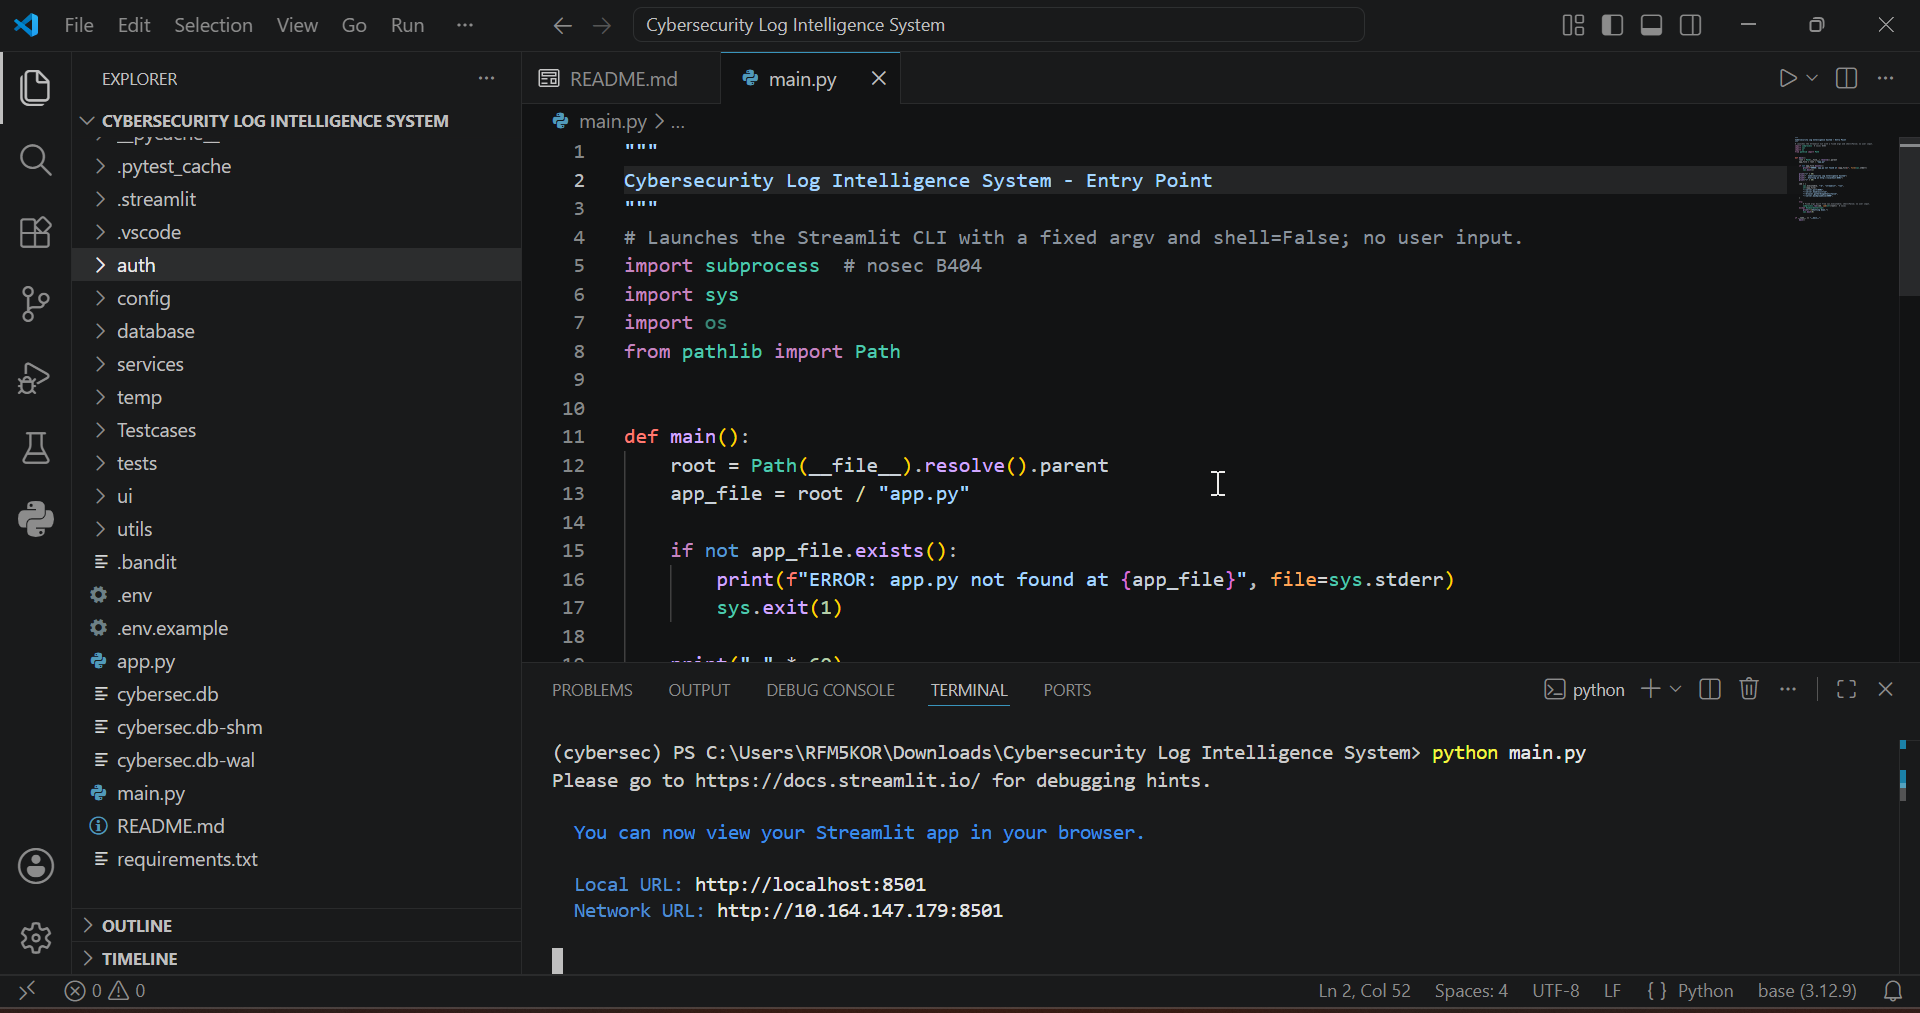
\includegraphics[width=0.69\textwidth]{vs.png}
\end{figure}

\subsection{Sign In Page}
\begin{figure}[H]
    \centering
    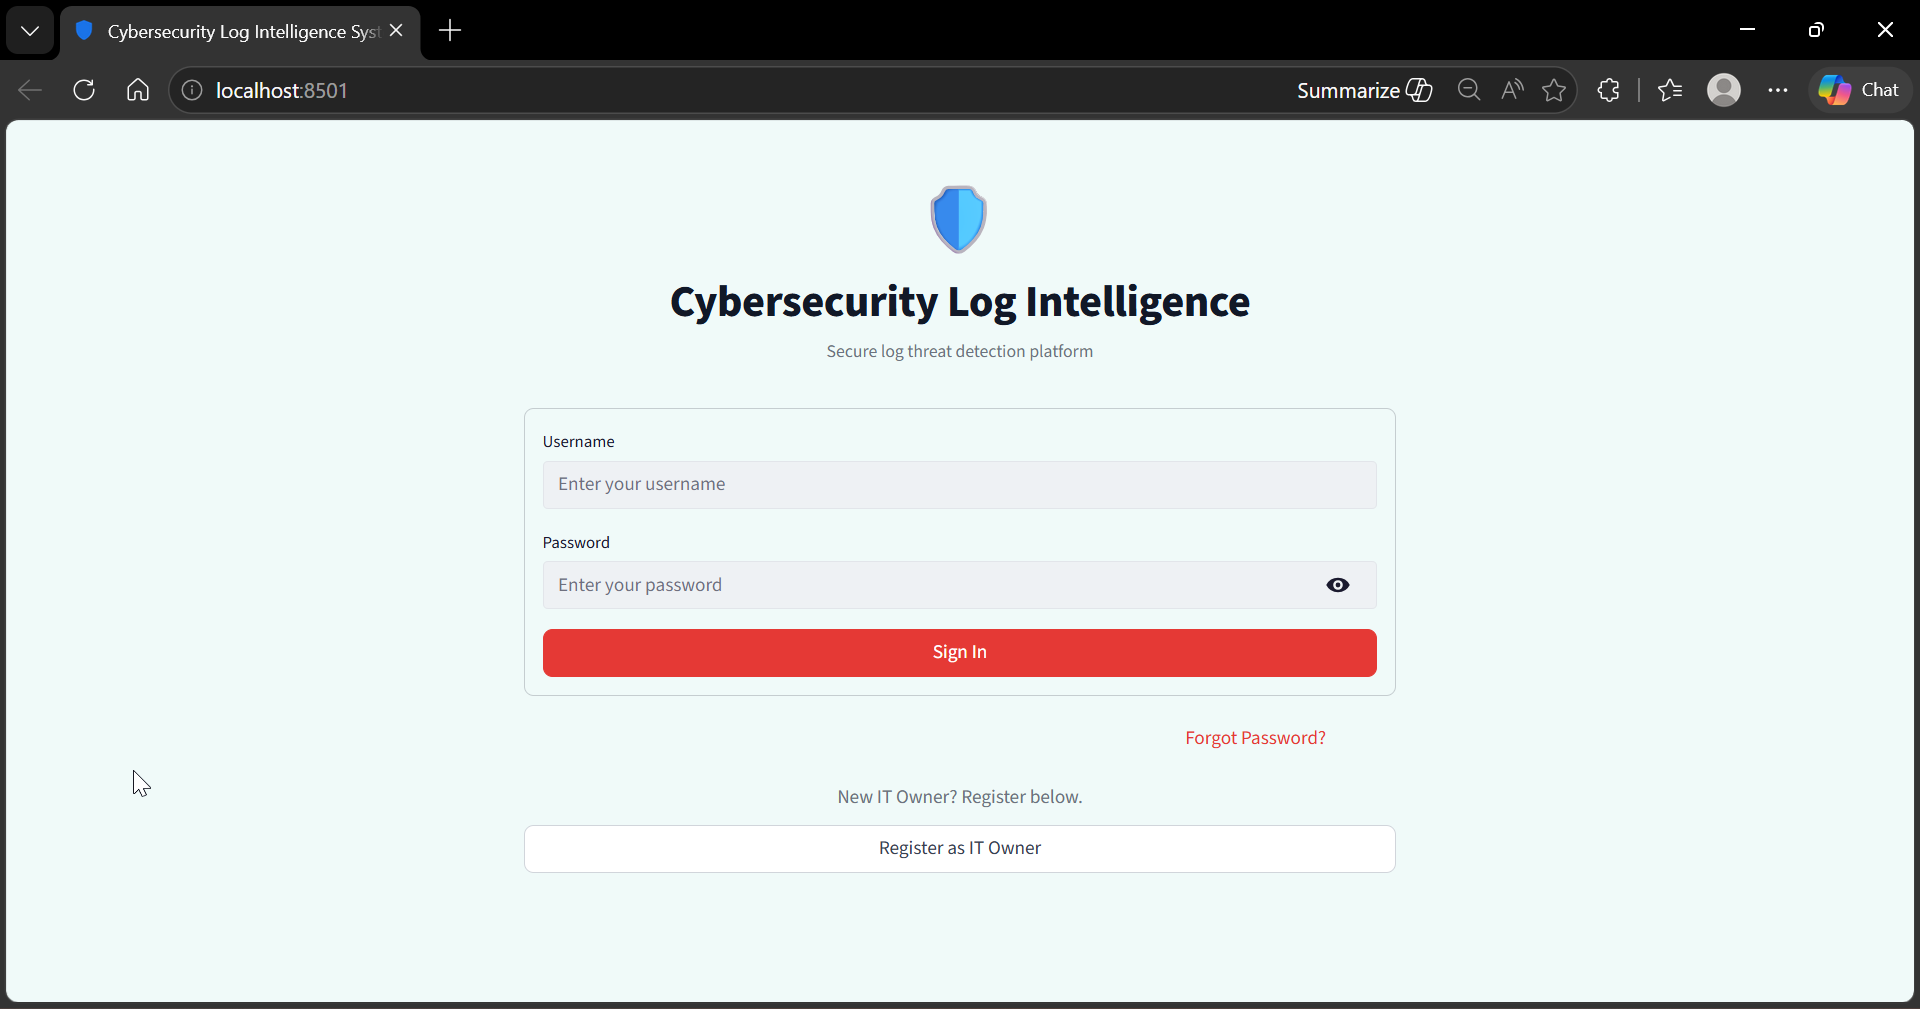
\includegraphics[width=0.69\textwidth]{login.png}
    \caption{Sign In/ Register interface}
    \label{fig:image}
\end{figure}

\subsection{Administrator Interface}
\subsubsection{Admin Homepage}
\begin{figure}[H]
    \centering
    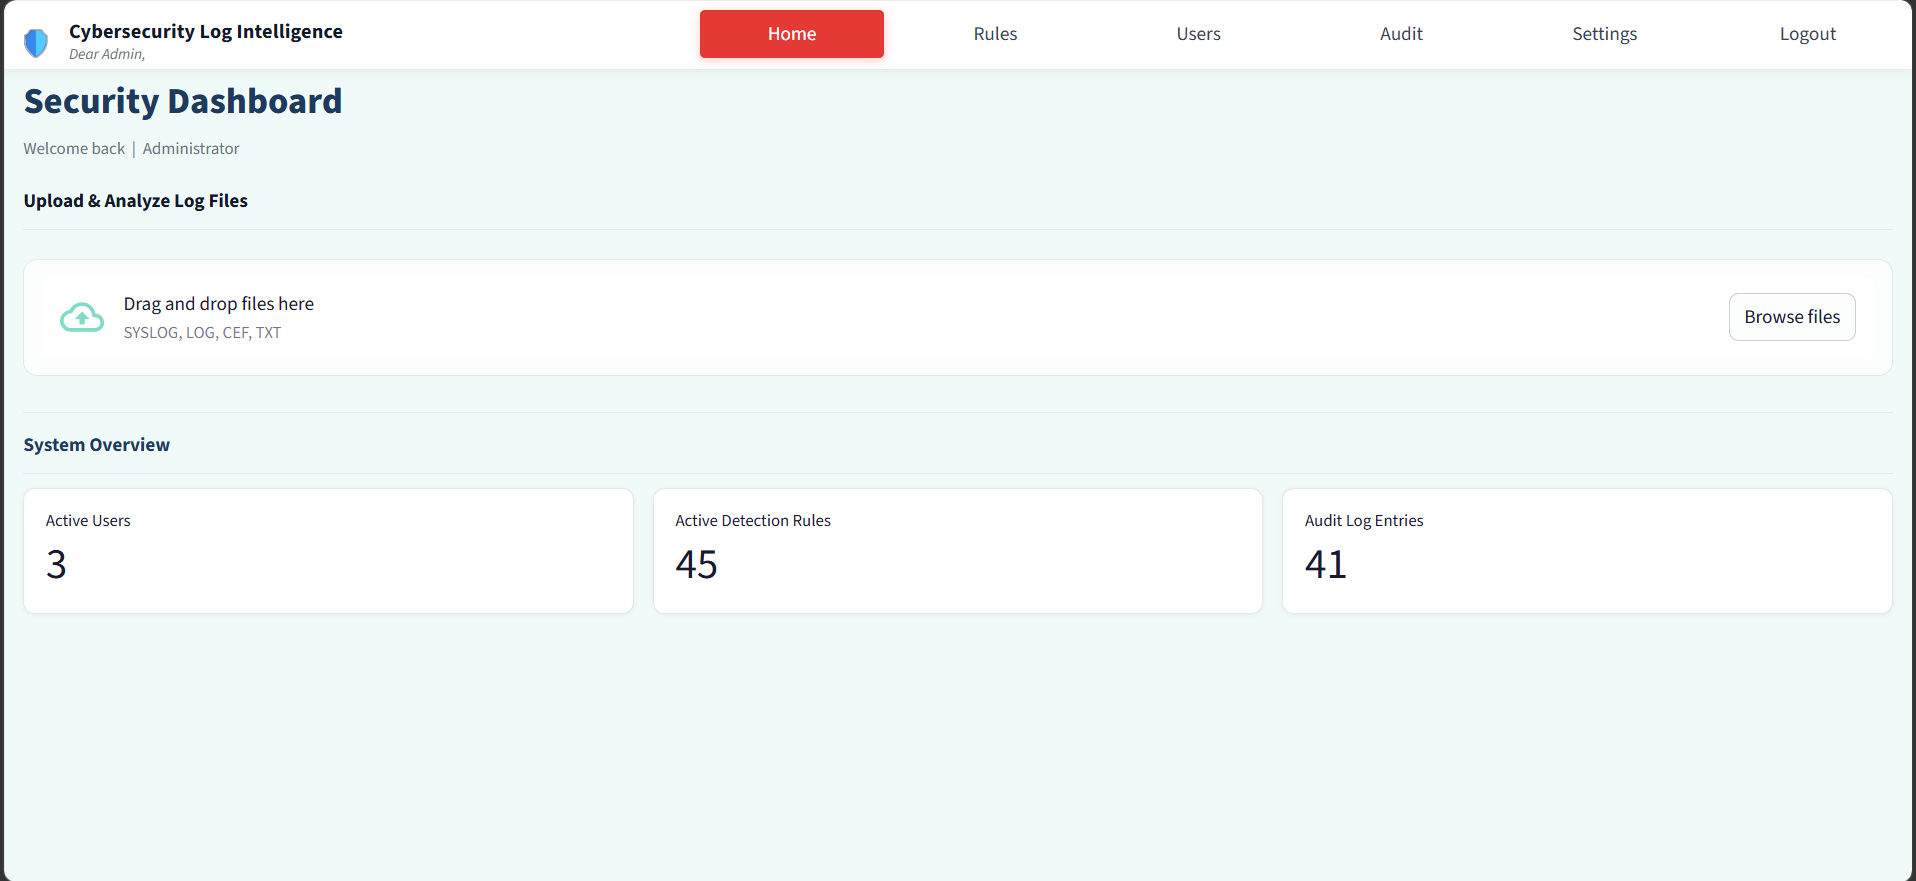
\includegraphics[width=0.69\textwidth]{admin_home.png}
    \caption{Admin Home with System Overview}
    \label{fig:image}
\end{figure}

\begin{figure}[H]
    \centering
    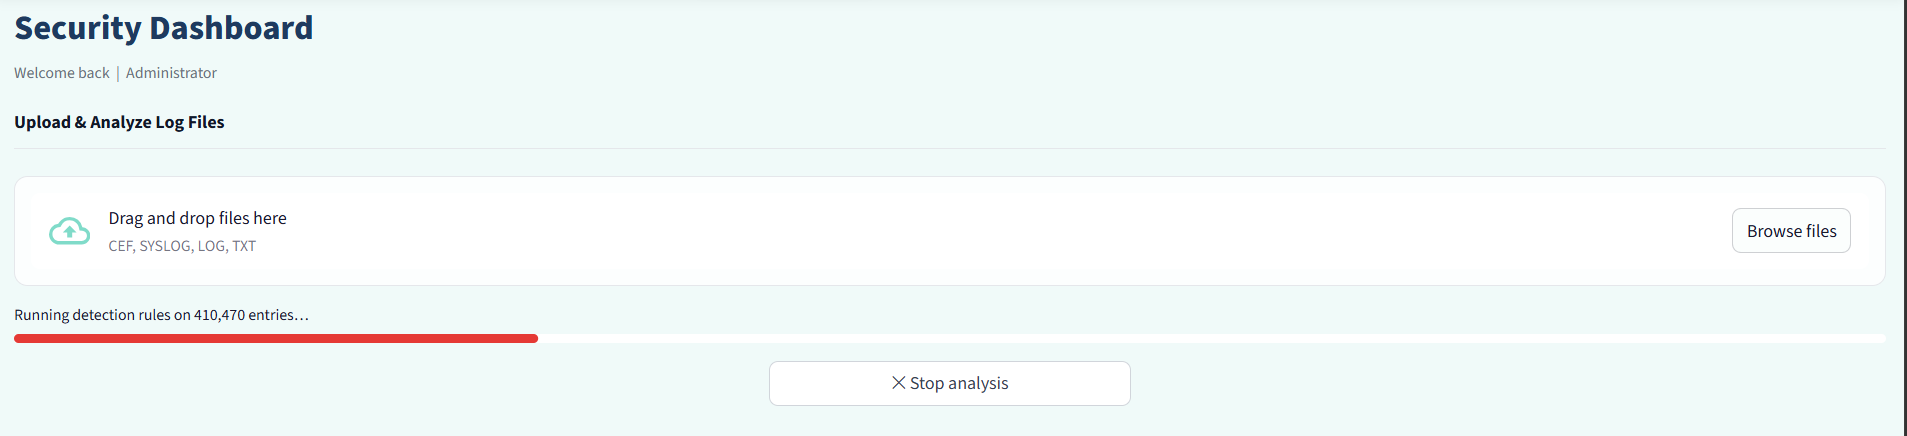
\includegraphics[width=0.69\textwidth]{admin_analysis.png}
    \caption{Admin Homepage during Log file analysis}
    \label{fig:image}
\end{figure}

\subsubsection{Admin Rules Page}
Admin can create, edit, enable, and disable the threat detection rules for all IT Owners
\begin{figure}[H]
    \centering
    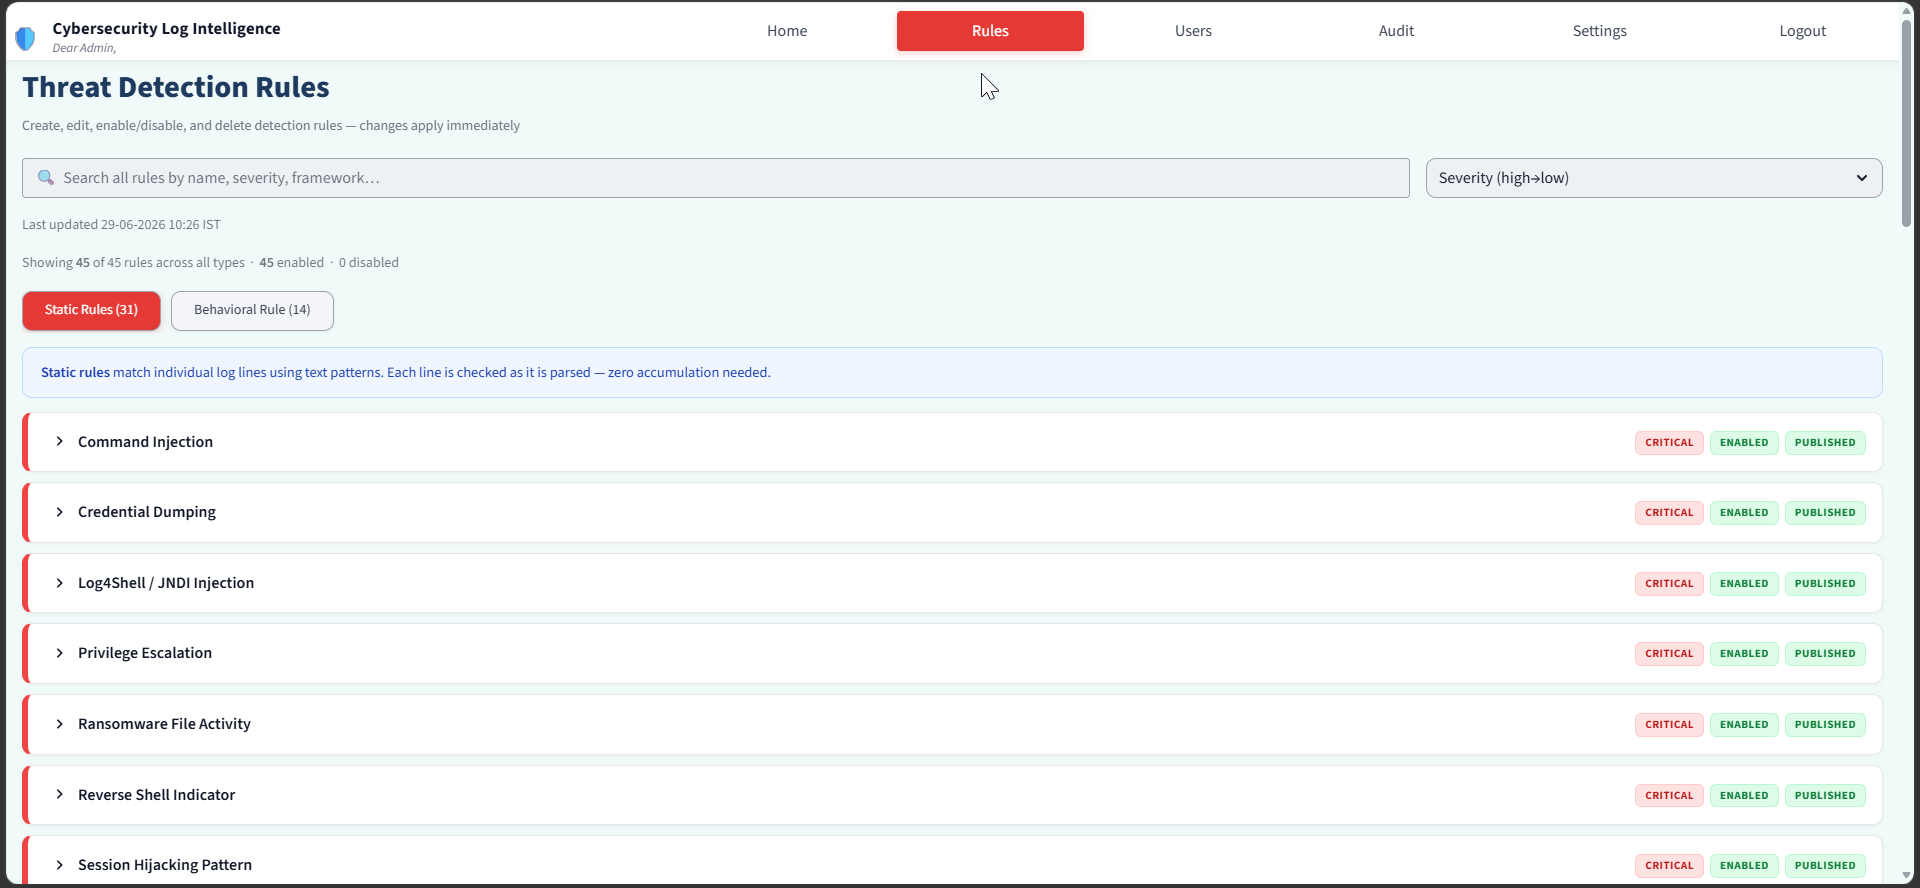
\includegraphics[width=0.75\textwidth]{admin_rule.png}
    \caption{All threat dectection rules with current status}
    \label{fig:image}
\end{figure}

\begin{figure}[H]
    \centering
    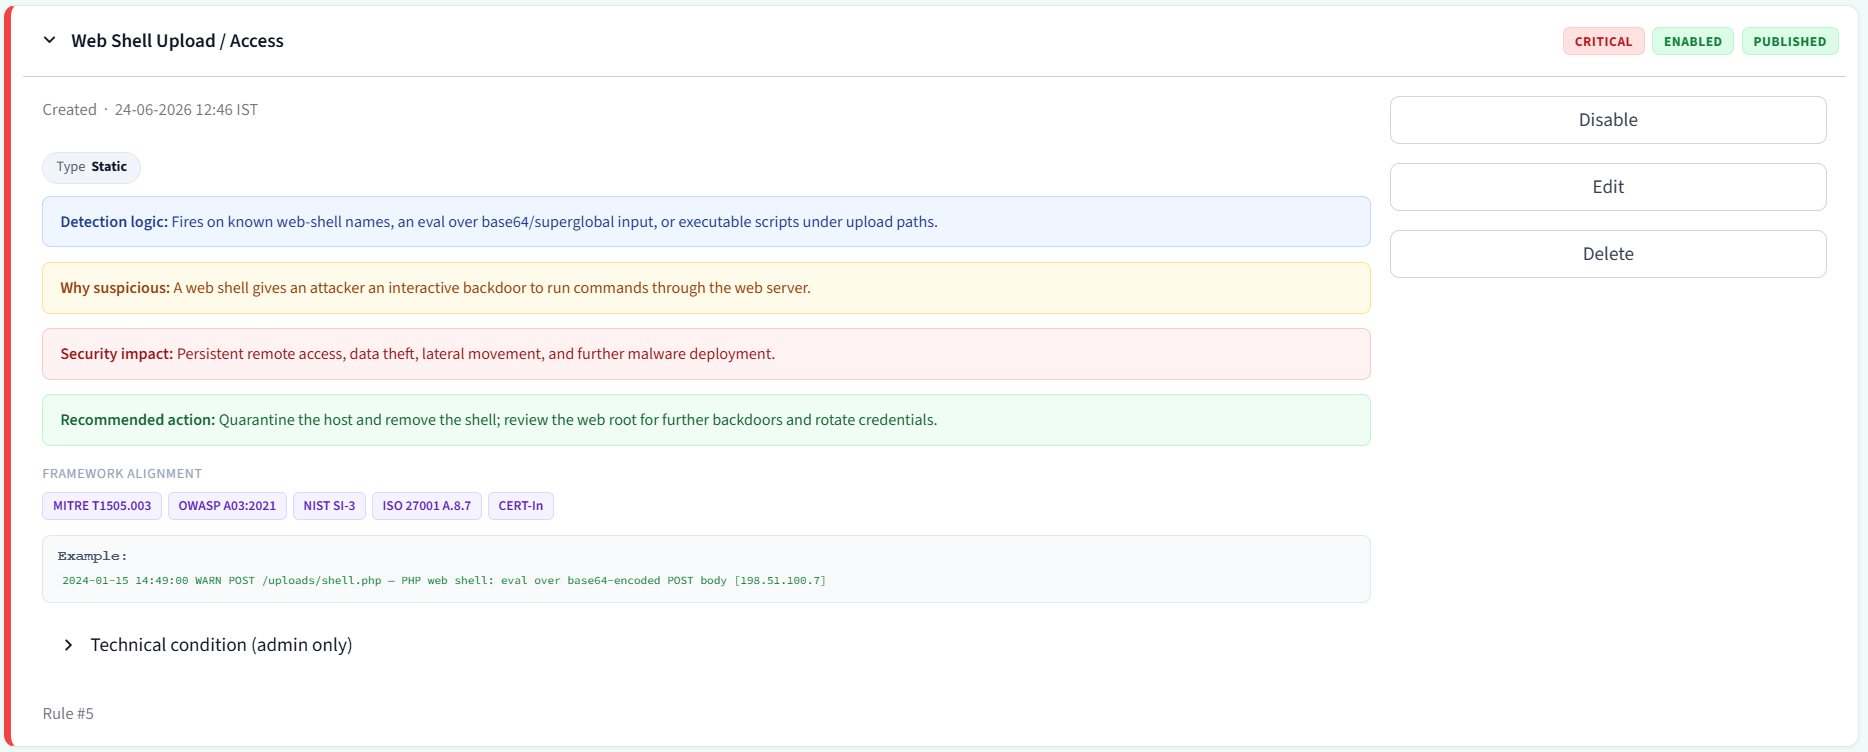
\includegraphics[width=0.75\textwidth]{admin_card.png}
    \caption{Configurable Threat detection rules}
    \label{fig:image}
\end{figure}

\begin{figure}[H]
    \centering
    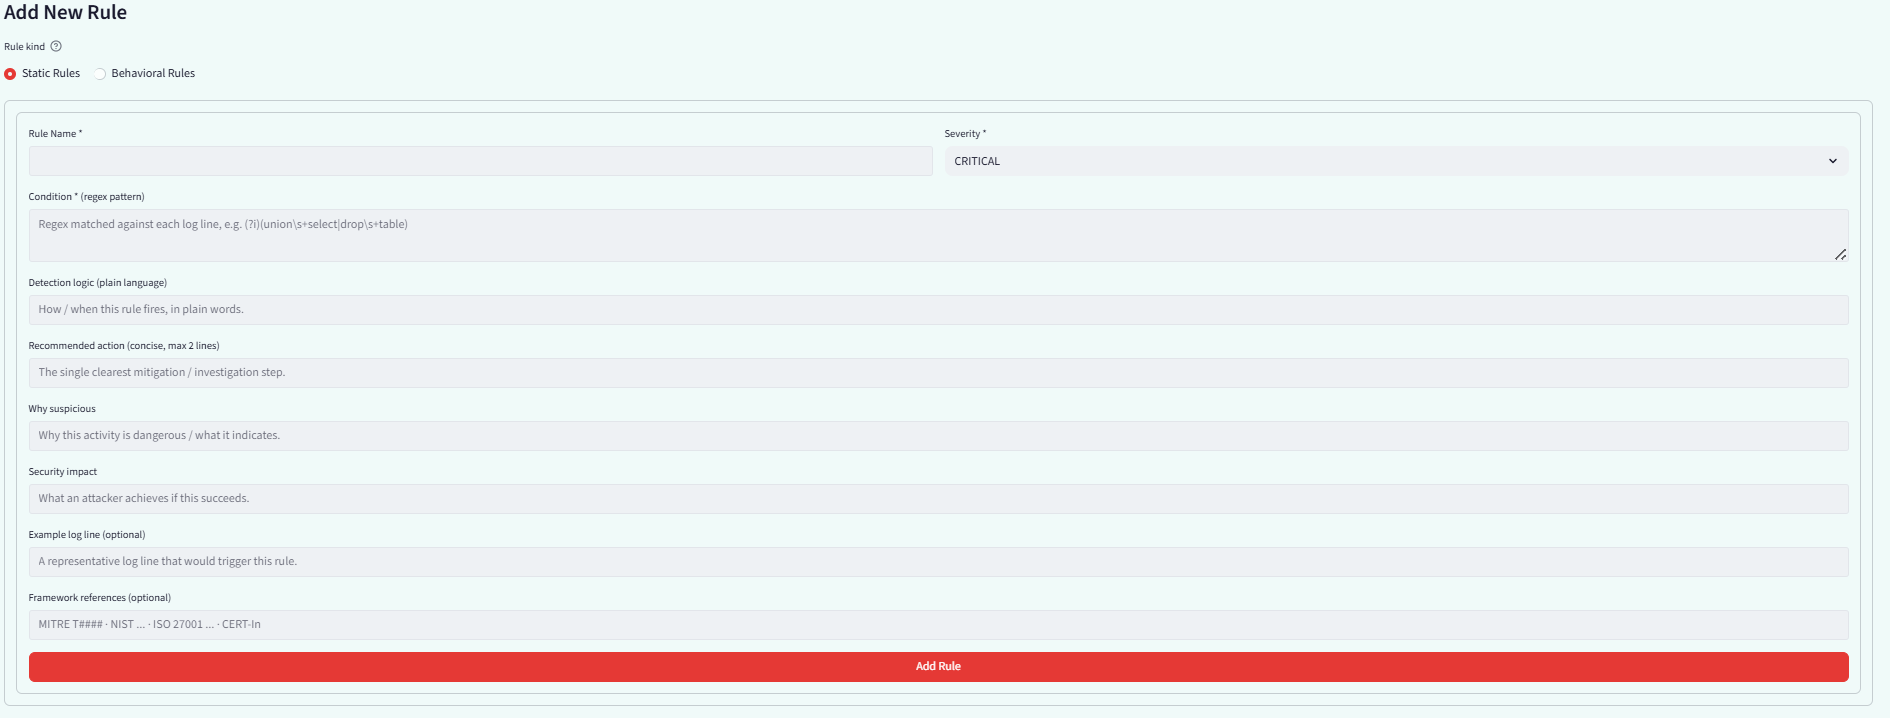
\includegraphics[width=0.75\textwidth]{create.png}
    \caption{Admin can add new Static/Behavioral rules}
    \label{fig:image}
\end{figure}

\newpage

\subsubsection{Admin Users Page}
\begin{figure}[H]
    \centering
    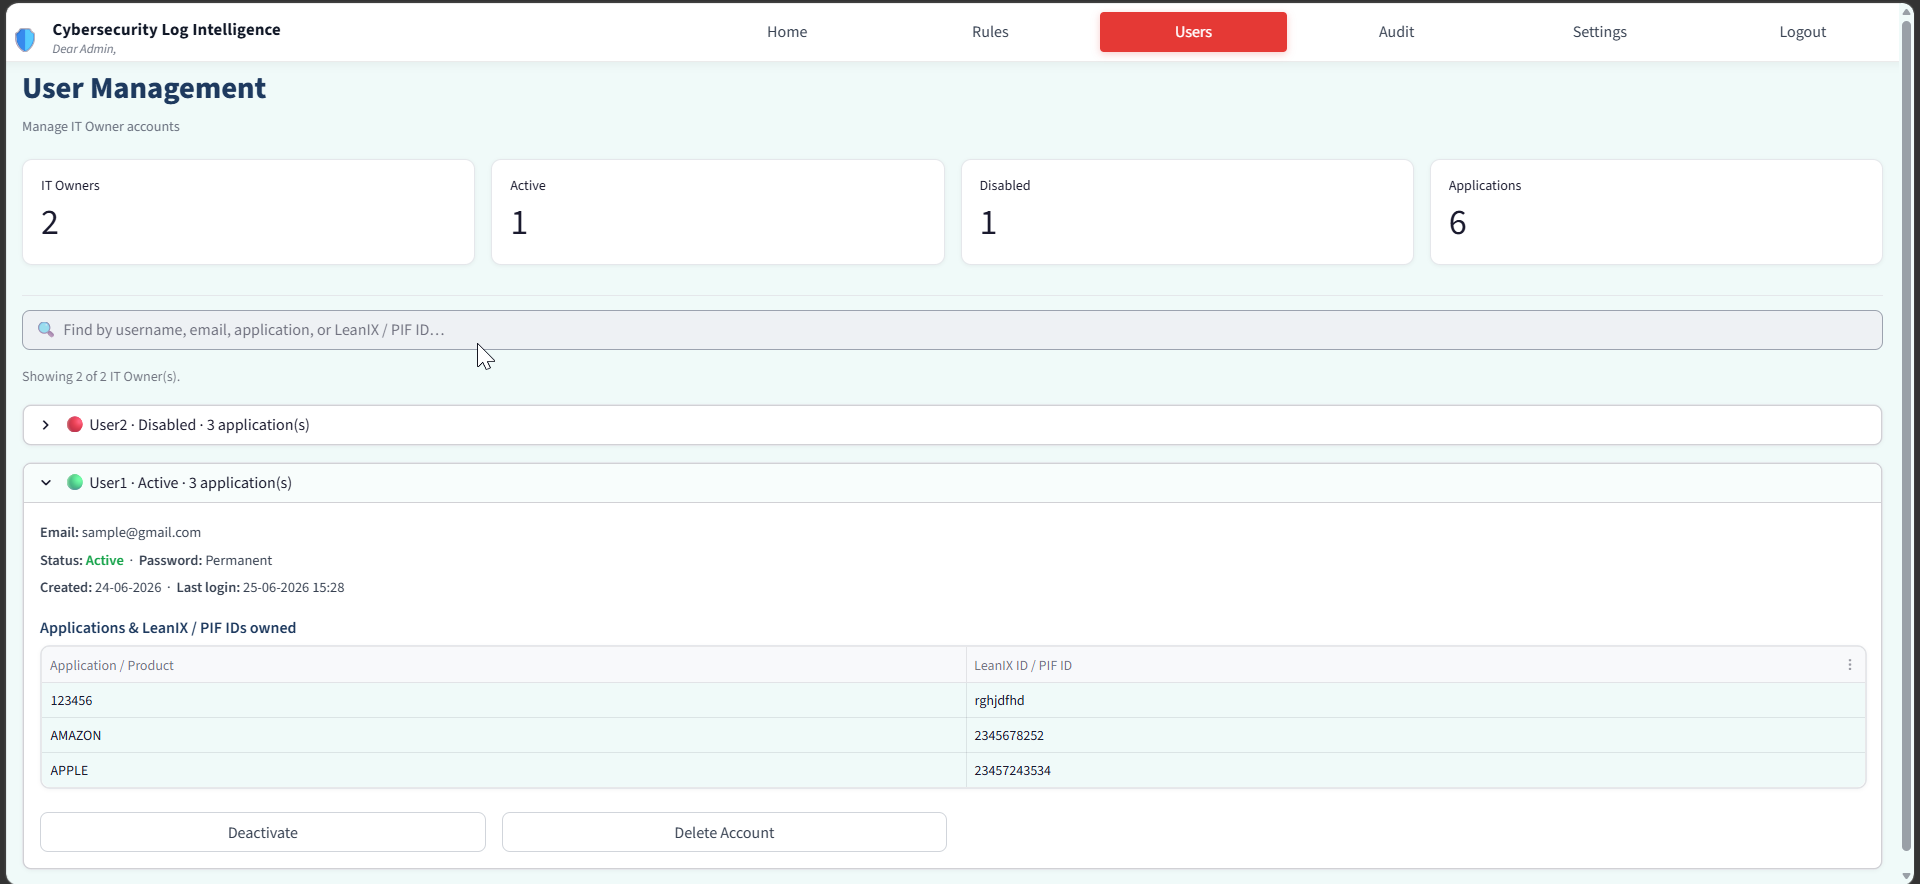
\includegraphics[width=0.8\textwidth]{admin_user.png}
    \caption{Admin can manage IT Owner's account}
    \label{fig:image}
\end{figure}

\subsubsection{Admin Audit Page}
\begin{figure}[H]
    \centering
    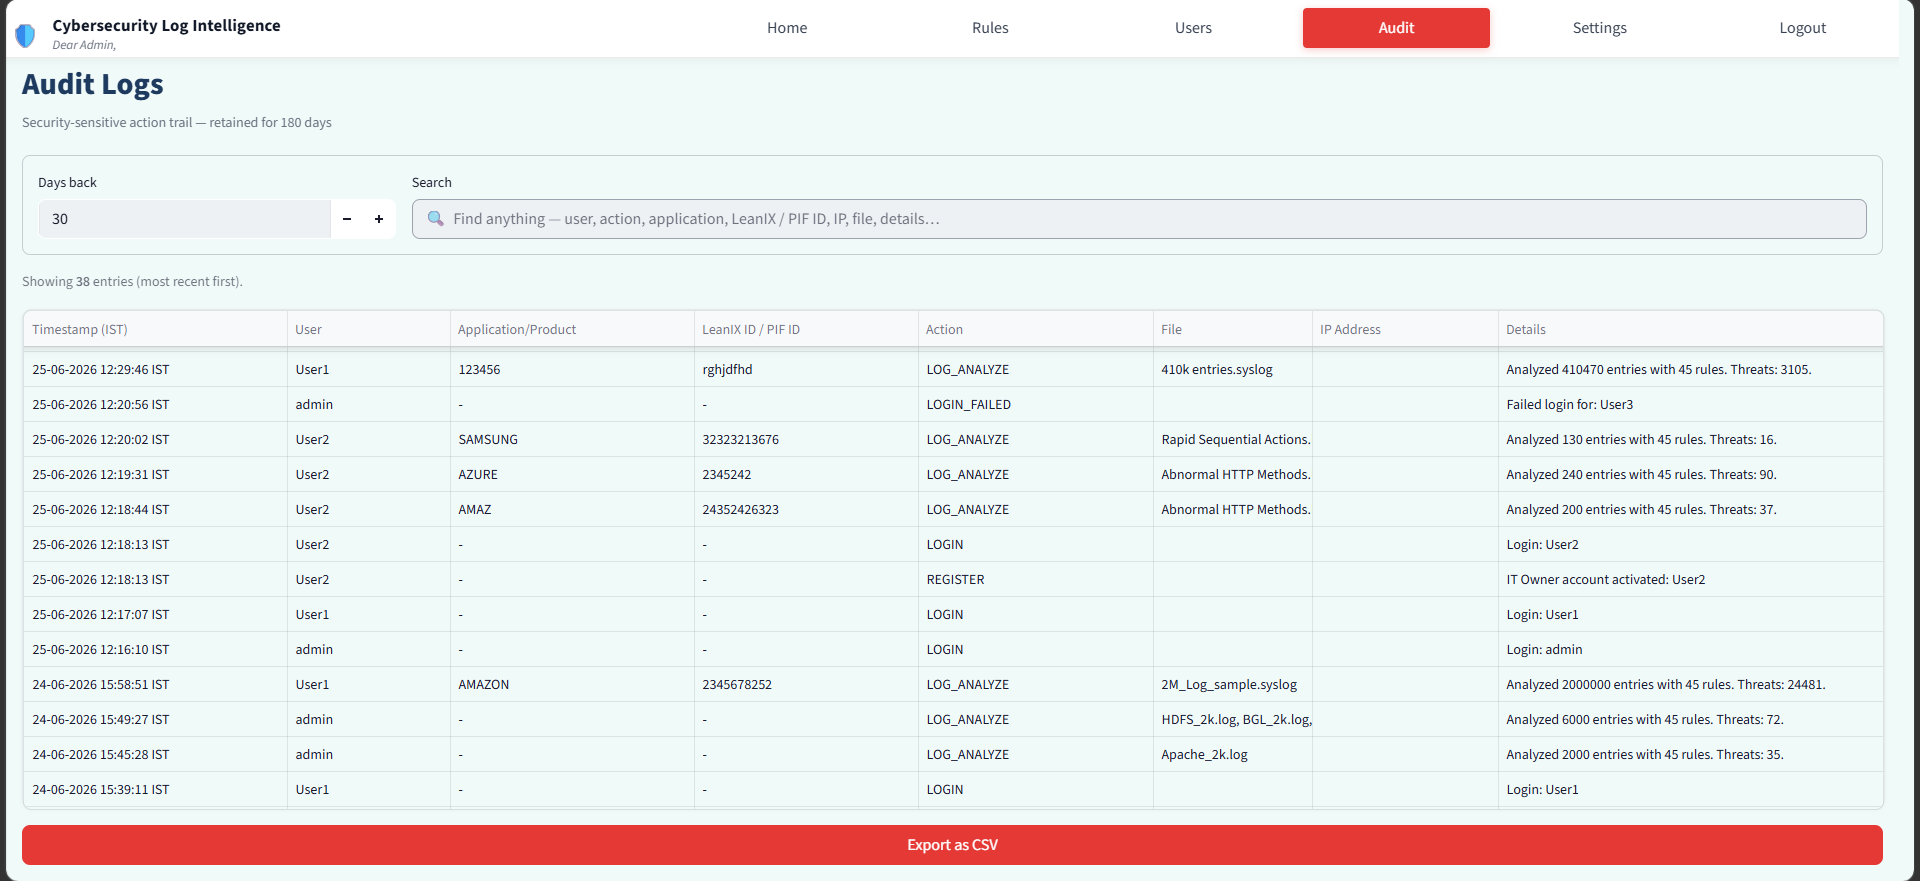
\includegraphics[width=0.8\textwidth]{admin_audit.png}
    \caption{Admin can view the application Logs}
    \label{fig:image}
\end{figure}

\subsubsection{Admin Settings Page}
\begin{figure}[H]
    \centering
    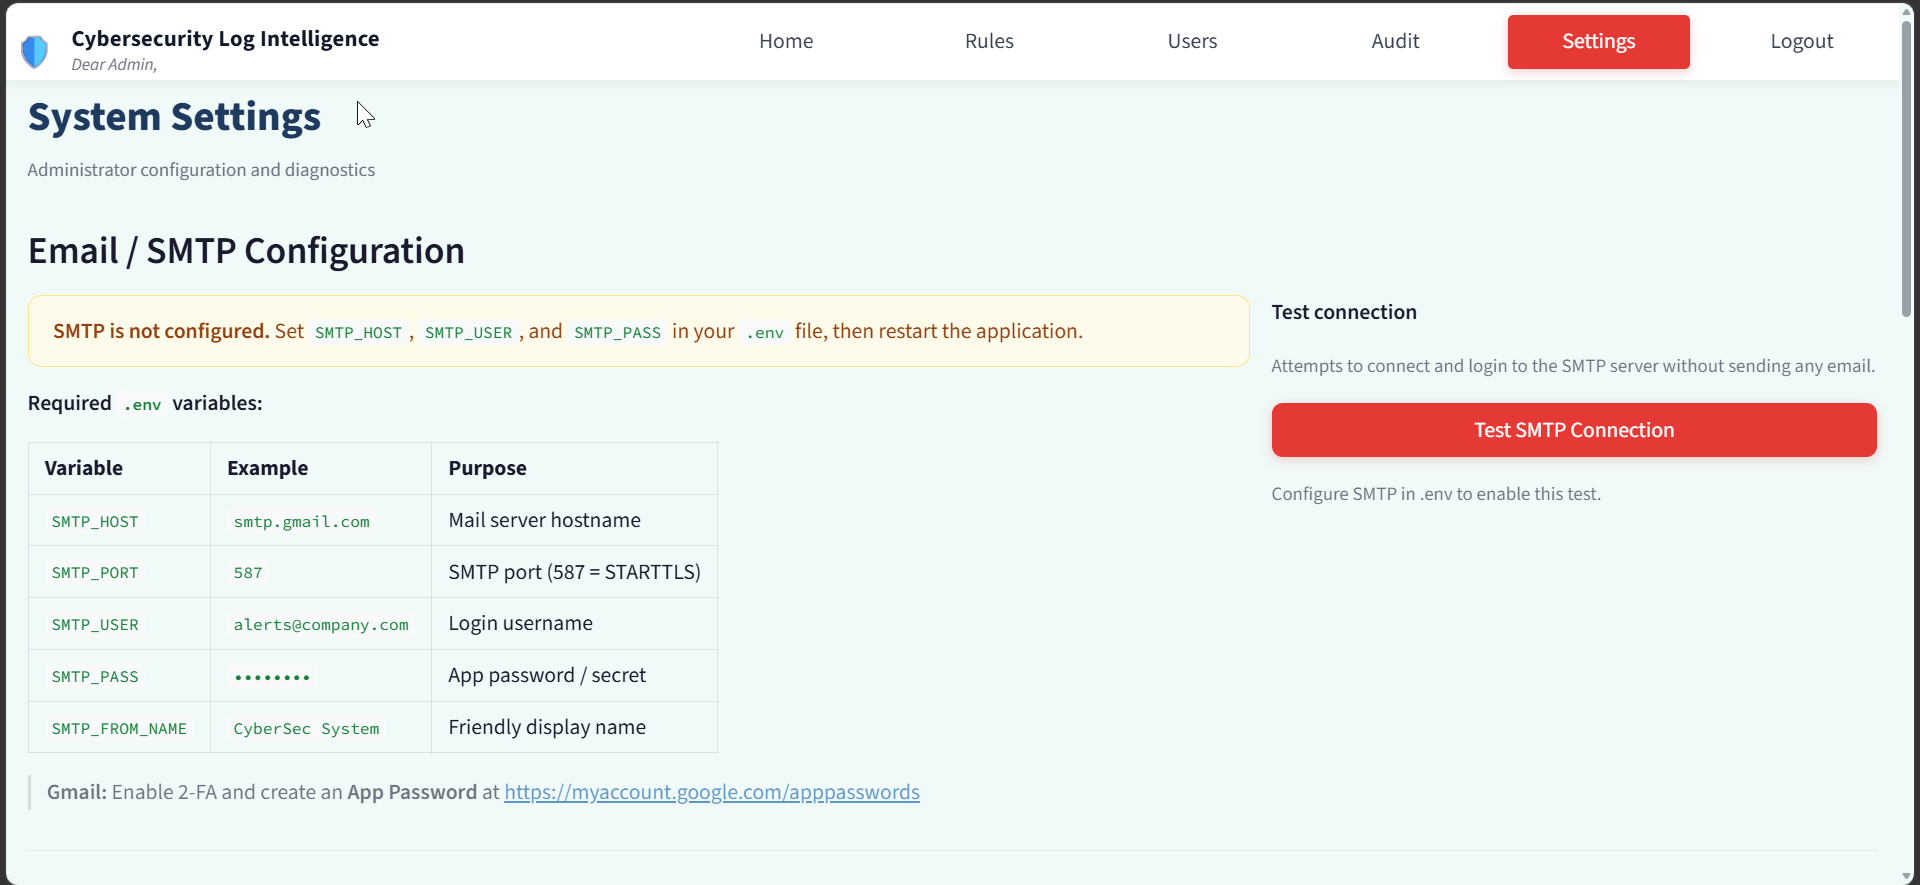
\includegraphics[width=0.8\textwidth]{admin_setting.png}
    \caption{Admin can test email, view active sessions, and update its account password}
    \label{fig:image}
\end{figure}


\newpage
\subsection{IT Owner Interface}
\subsubsection{IT Owner Home Page}

\begin{figure}[H]
    \centering
    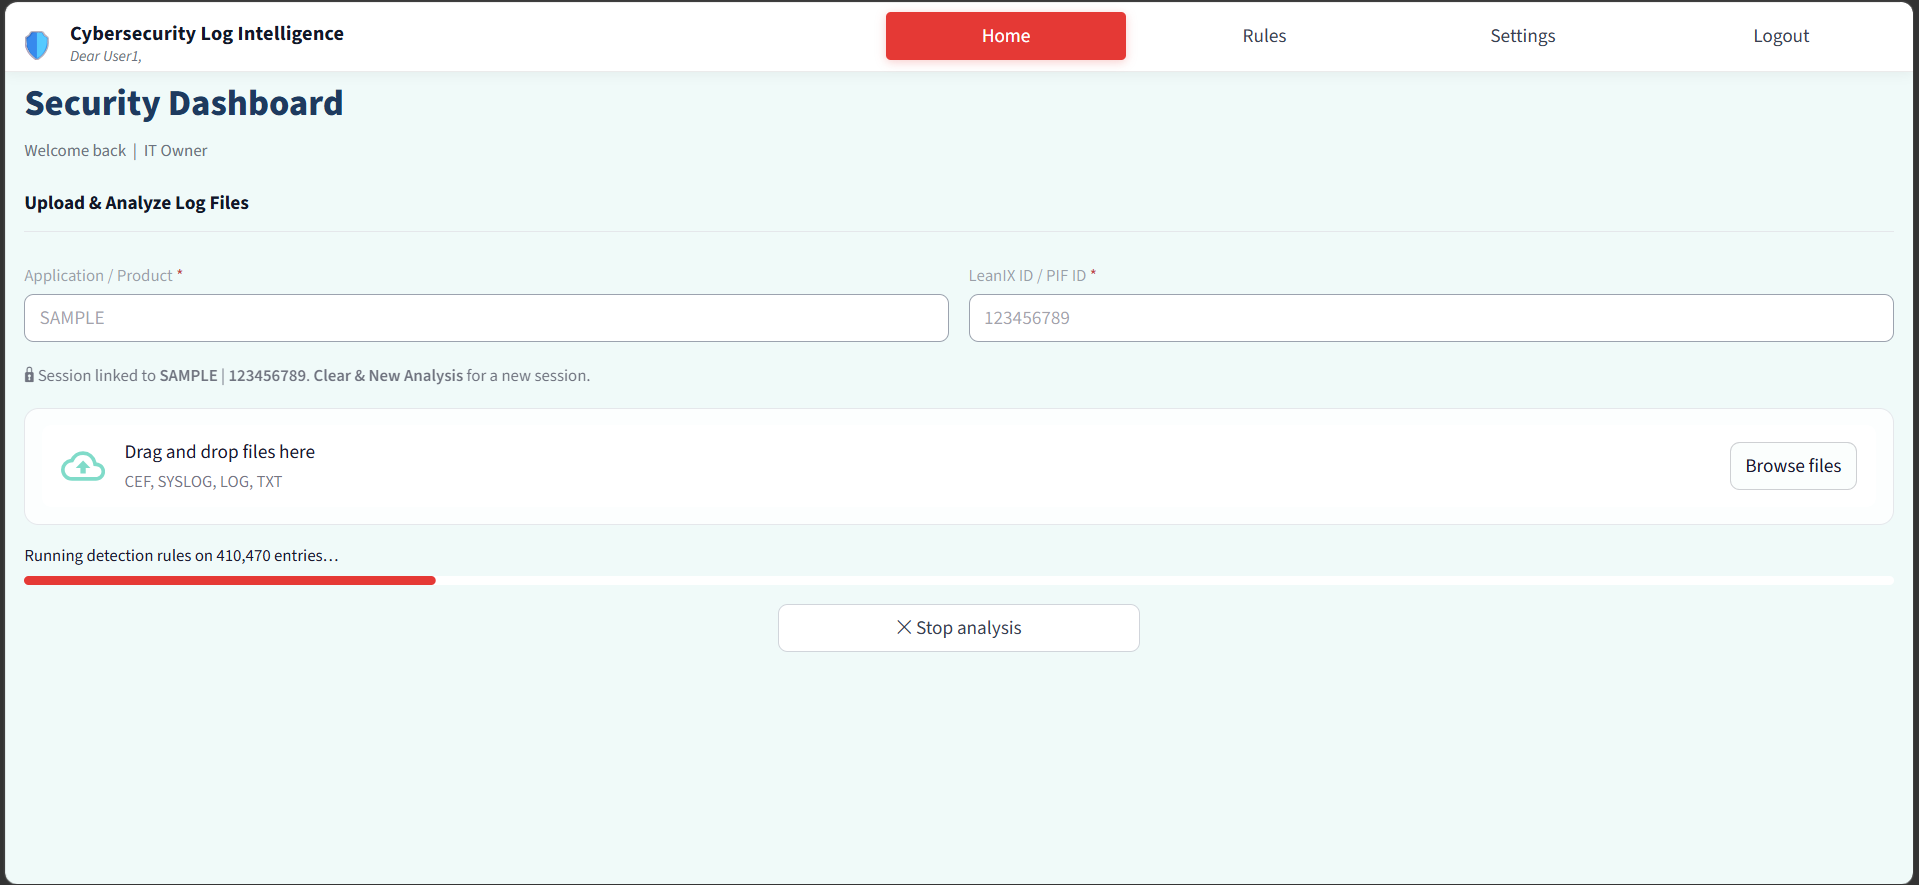
\includegraphics[width=0.85\textwidth]{user_home.png}
    \caption{Application/Product and LeanIX ID/PIF ID must be provided by all IT Owners before initiating log file analysis.}
    \label{fig:image}
\end{figure}

\subsubsection{IT Owner Rules Page}

\begin{figure}[H]
    \centering
    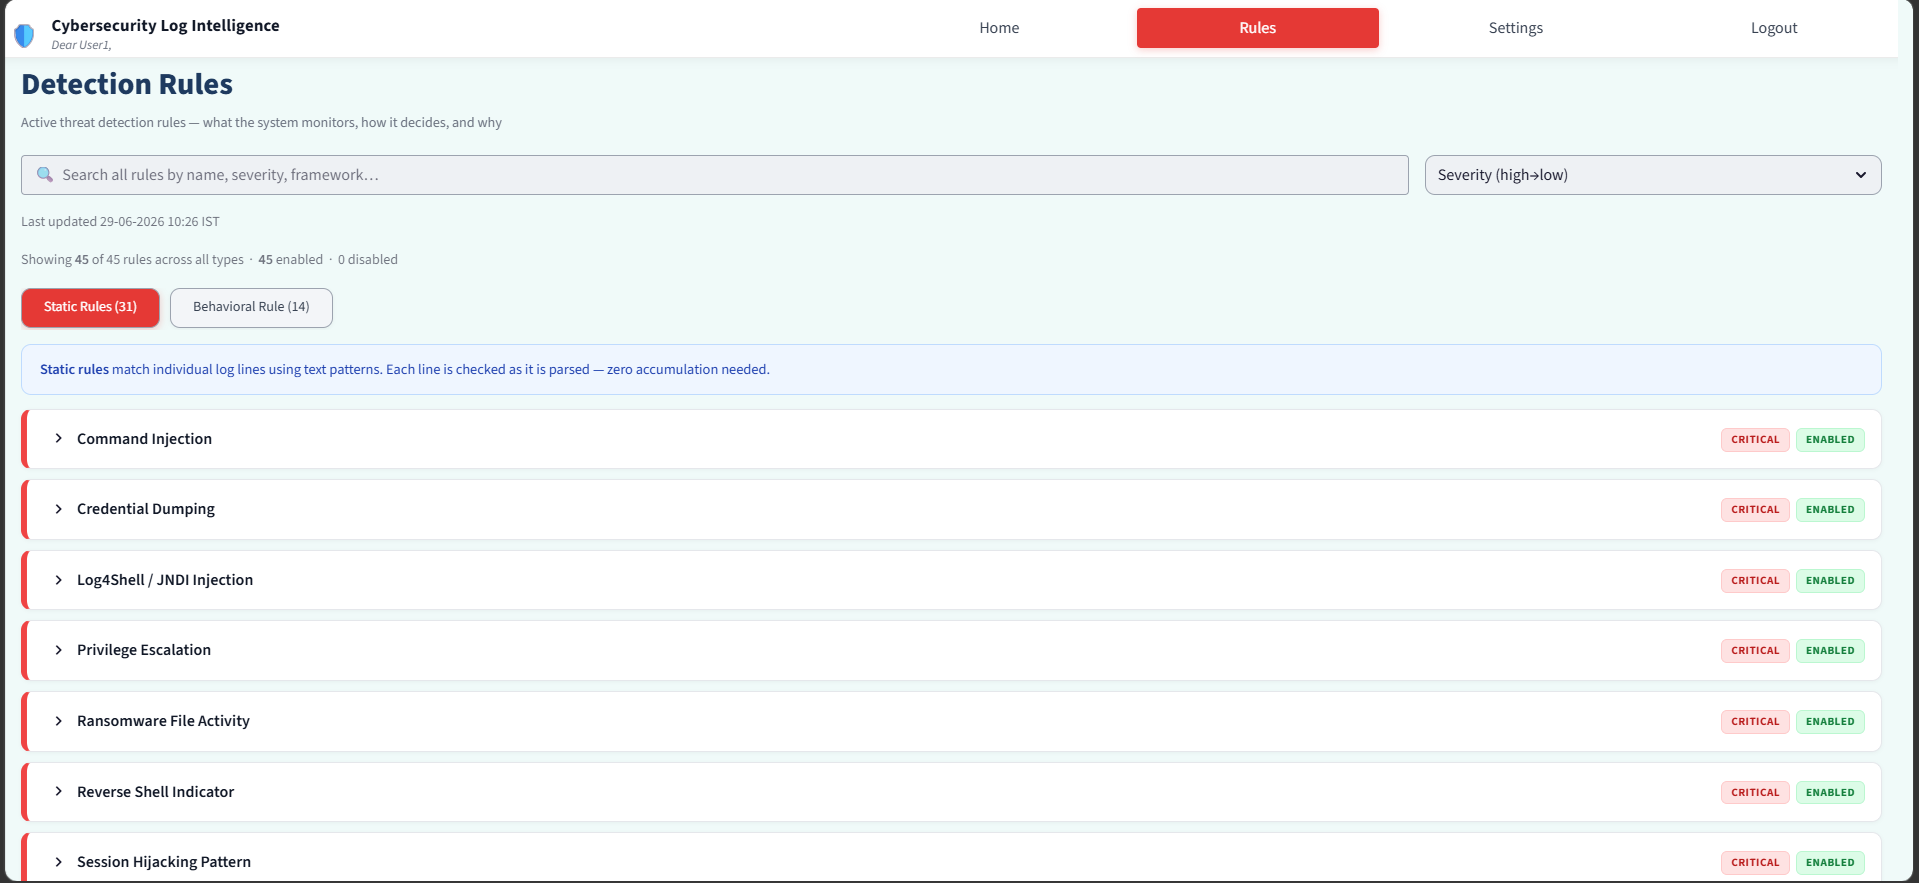
\includegraphics[width=0.85\textwidth]{user_rule.png}
\end{figure}

\begin{figure}[H]
    \centering
    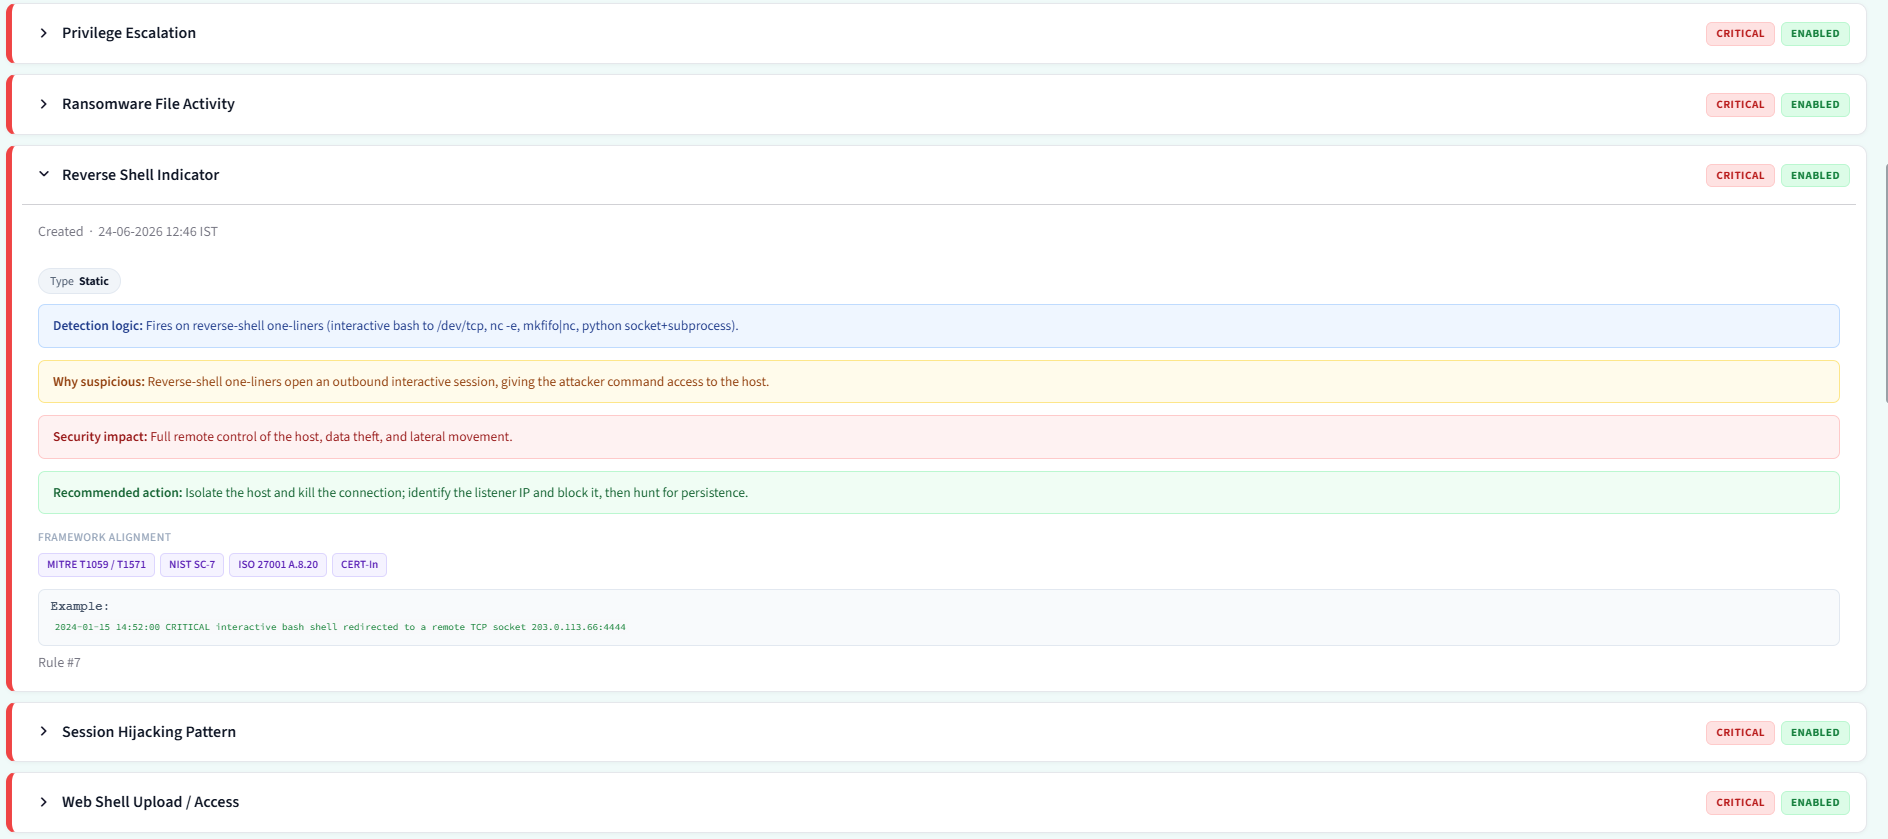
\includegraphics[width=0.85\textwidth]{user_card.png}
    \caption{IT Owners can only view the Threat detection rules}
    \label{fig:image}
\end{figure}


\newpage
\subsubsection{IT Owner Settings Page}

\begin{figure}[H]
    \centering
    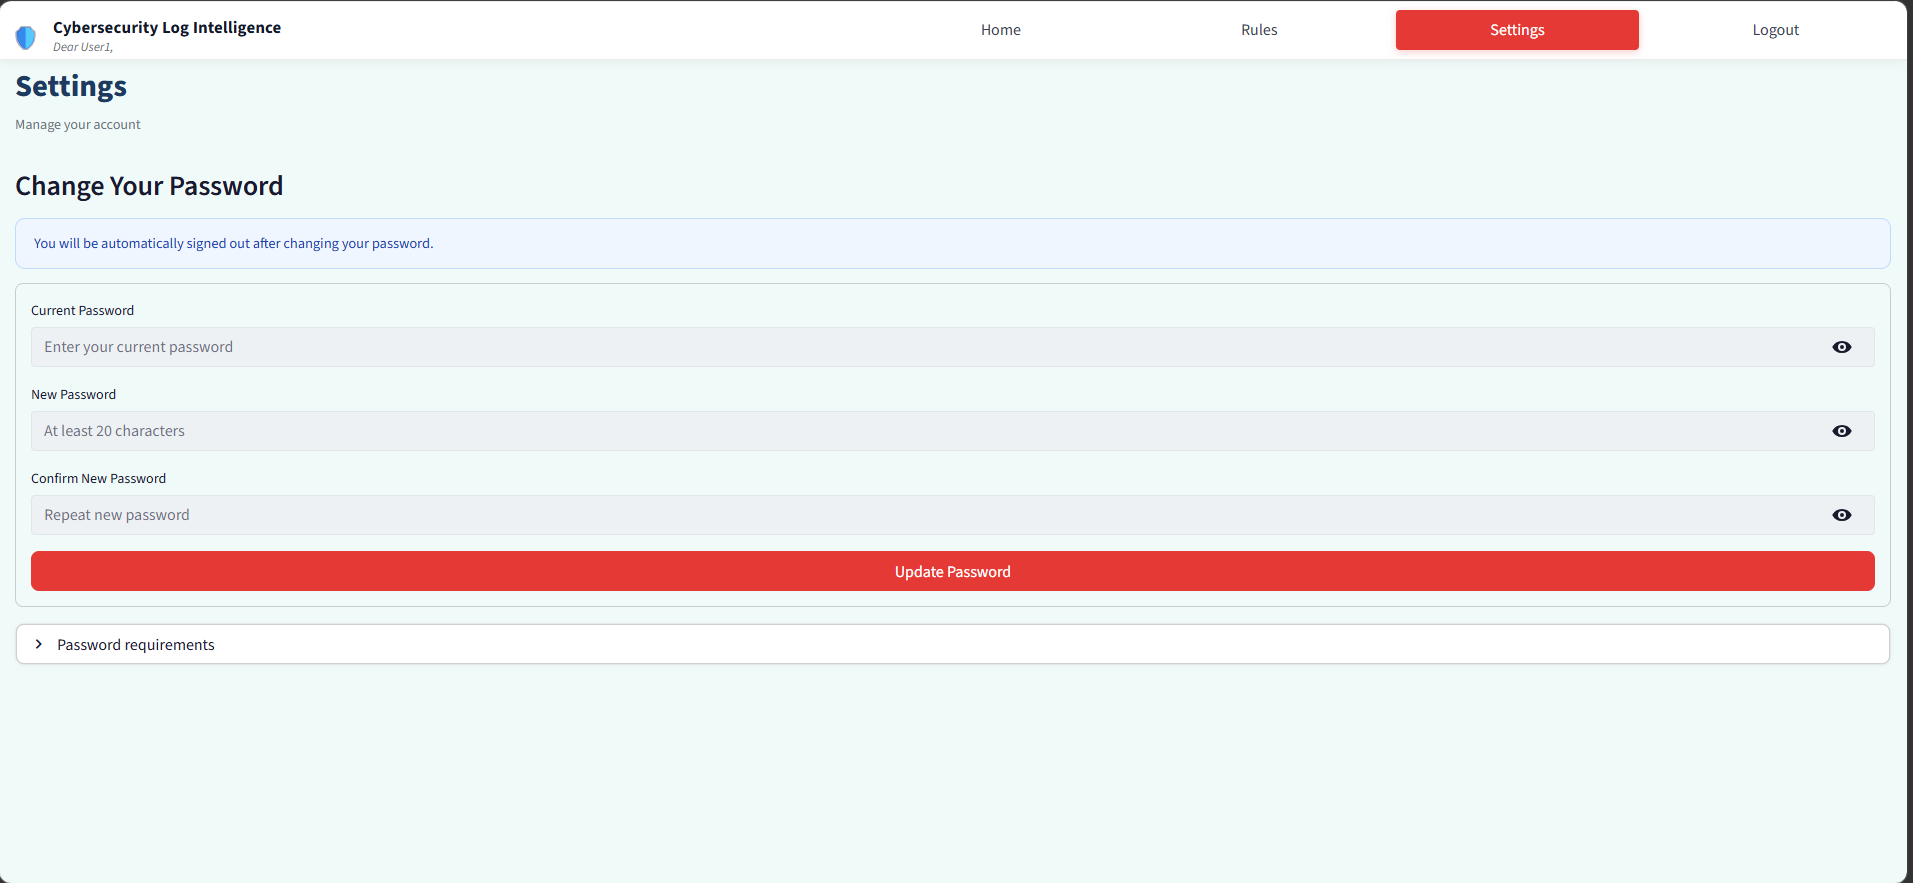
\includegraphics[width=0.92\textwidth]{user_setting.png}
    \caption{IT Owners can update its account password}
    \label{fig:image}
\end{figure}

\subsection{Log Analysis Output}
\subsubsection{Visualizations}
\begin{figure}[H]
    \centering
    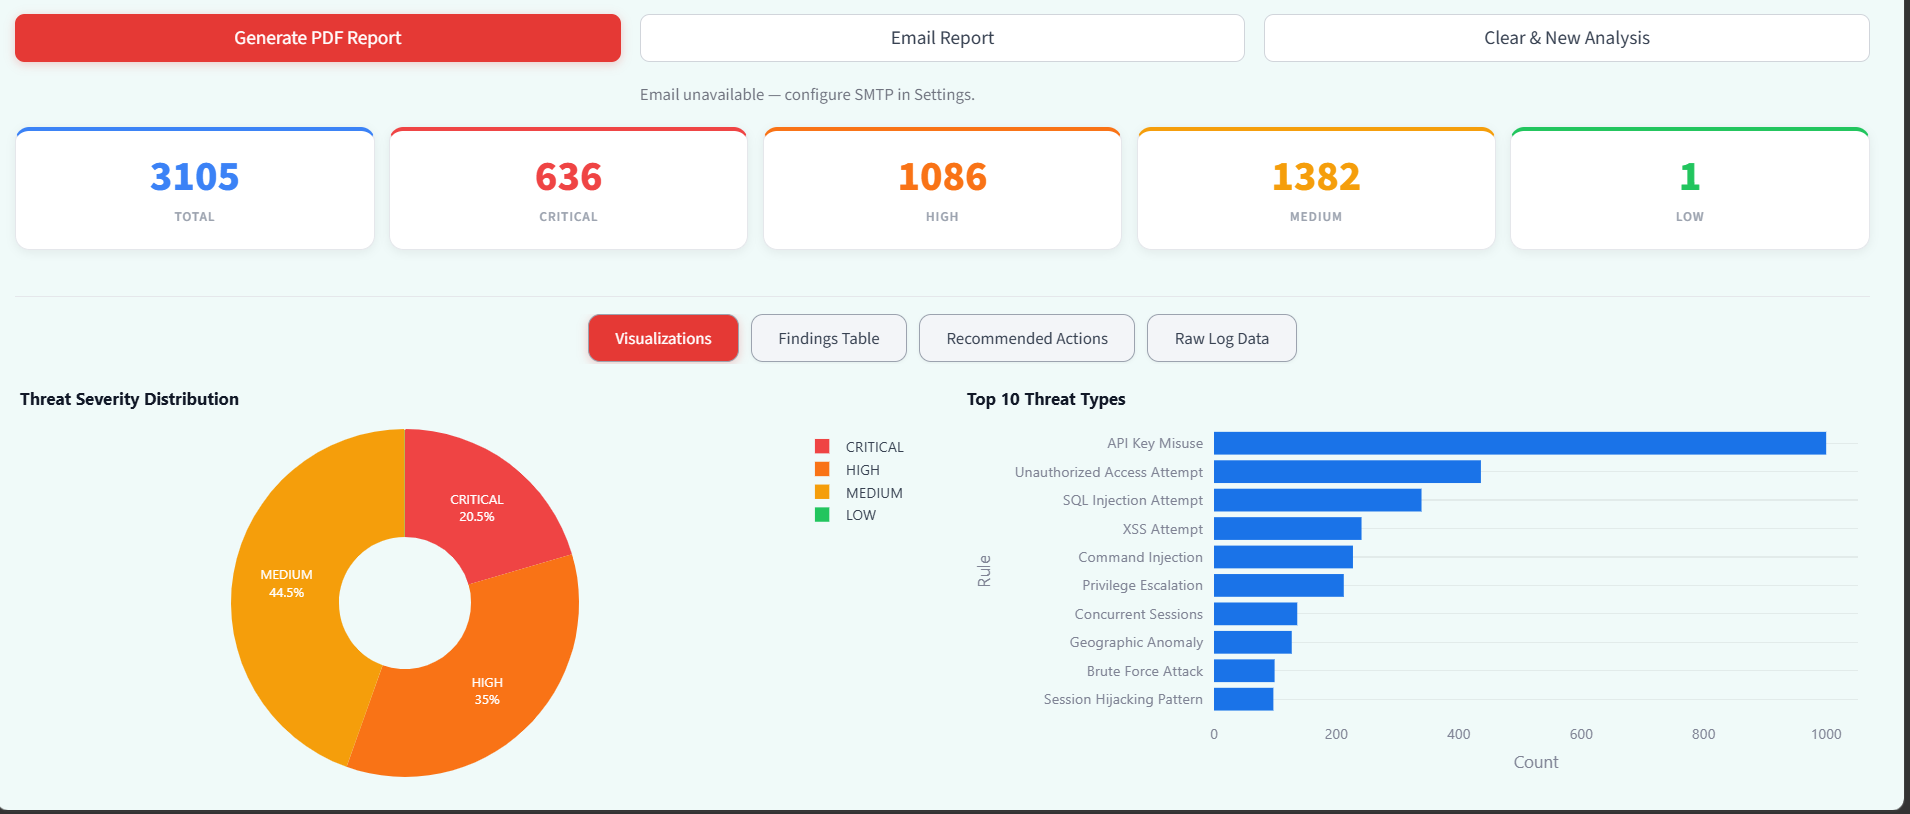
\includegraphics[width=0.92\textwidth]{plot0.png}
\end{figure}

\begin{figure}[H]
    \centering
    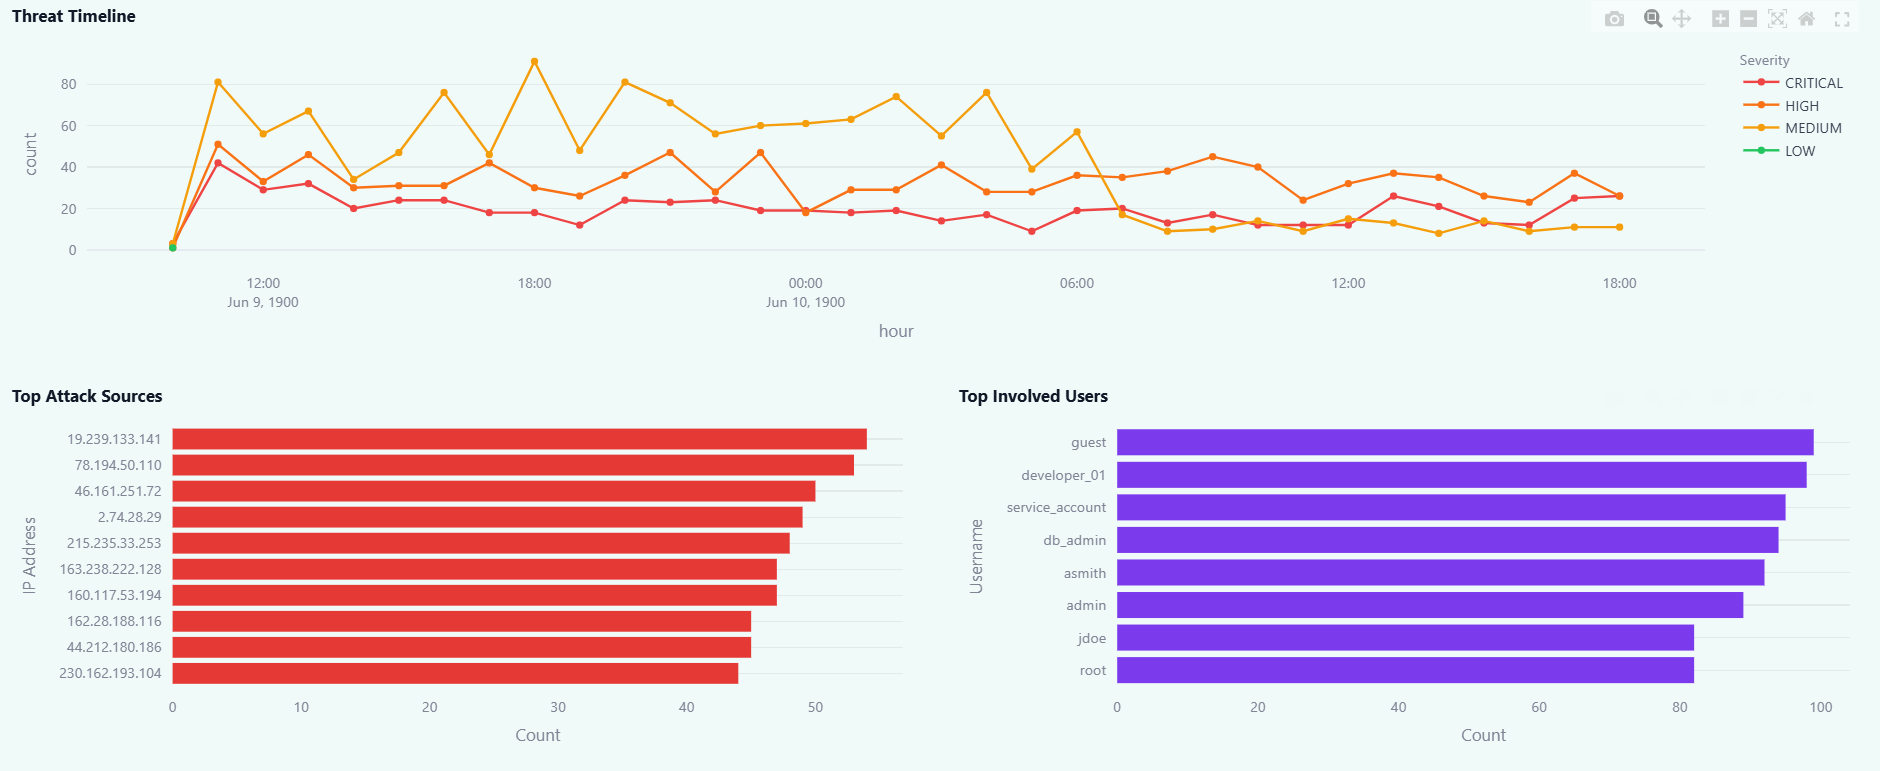
\includegraphics[width=0.92\textwidth]{plot.png}
\end{figure}
\newpage
\begin{figure}[H]
    \centering
    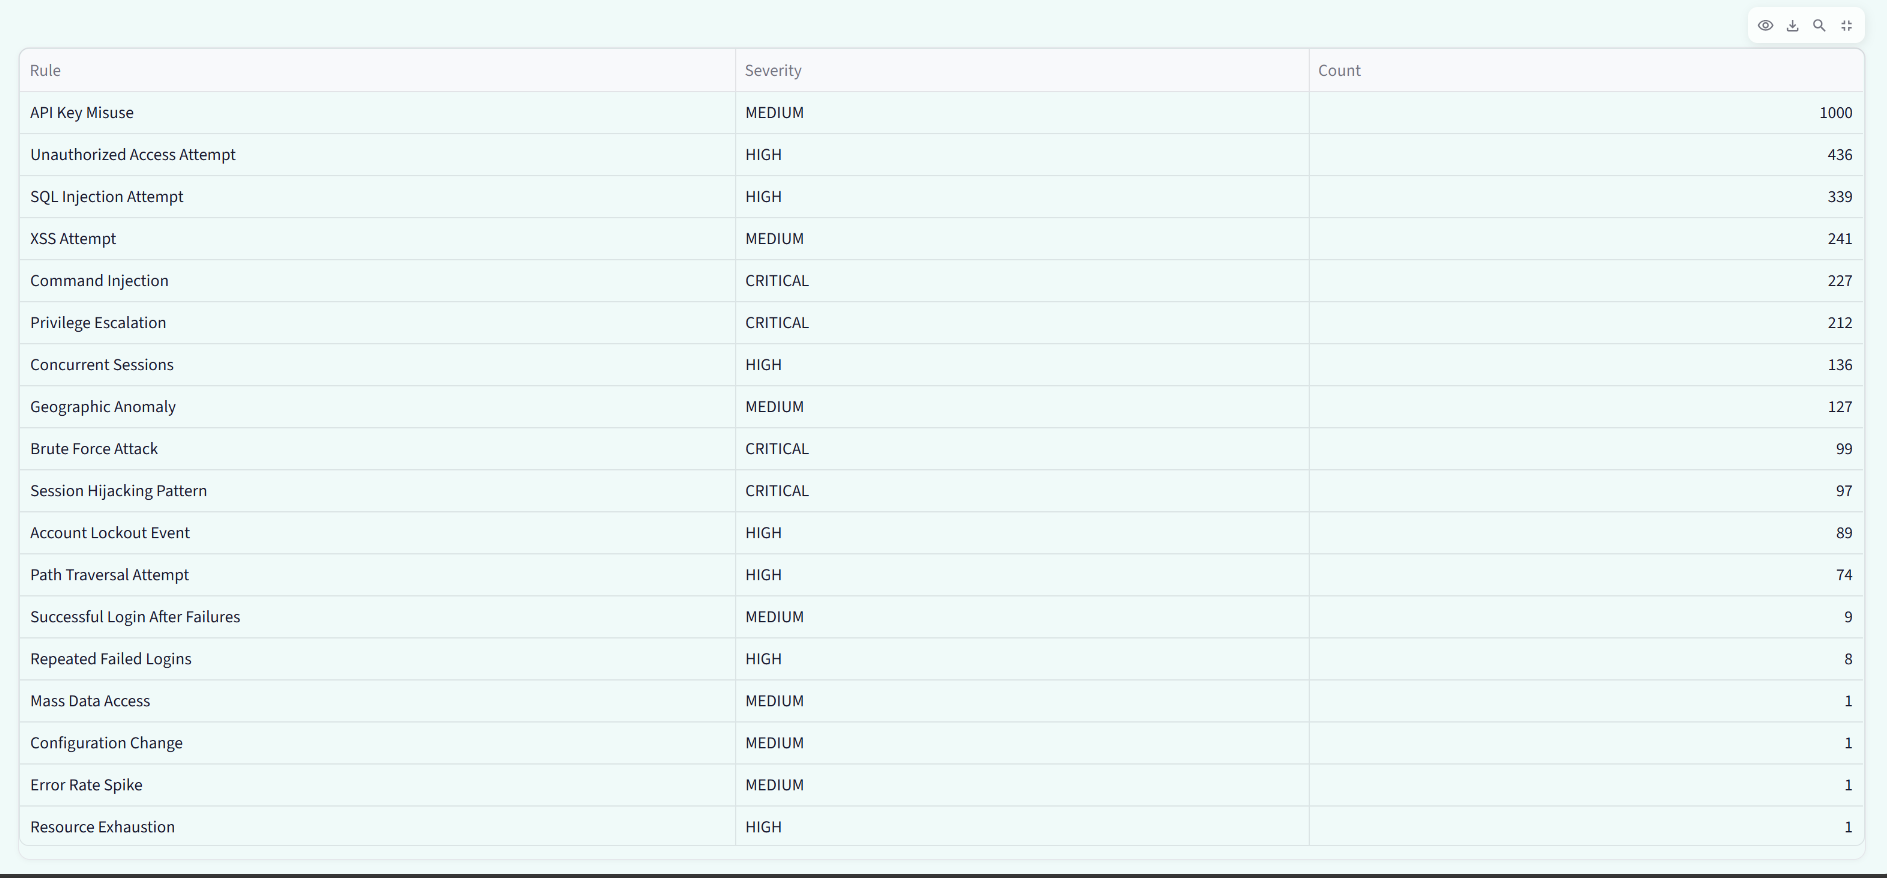
\includegraphics[width=0.92\textwidth]{rule_table.png}
\end{figure}

\subsubsection{Findings Table}
\begin{figure}[H]
    \centering
    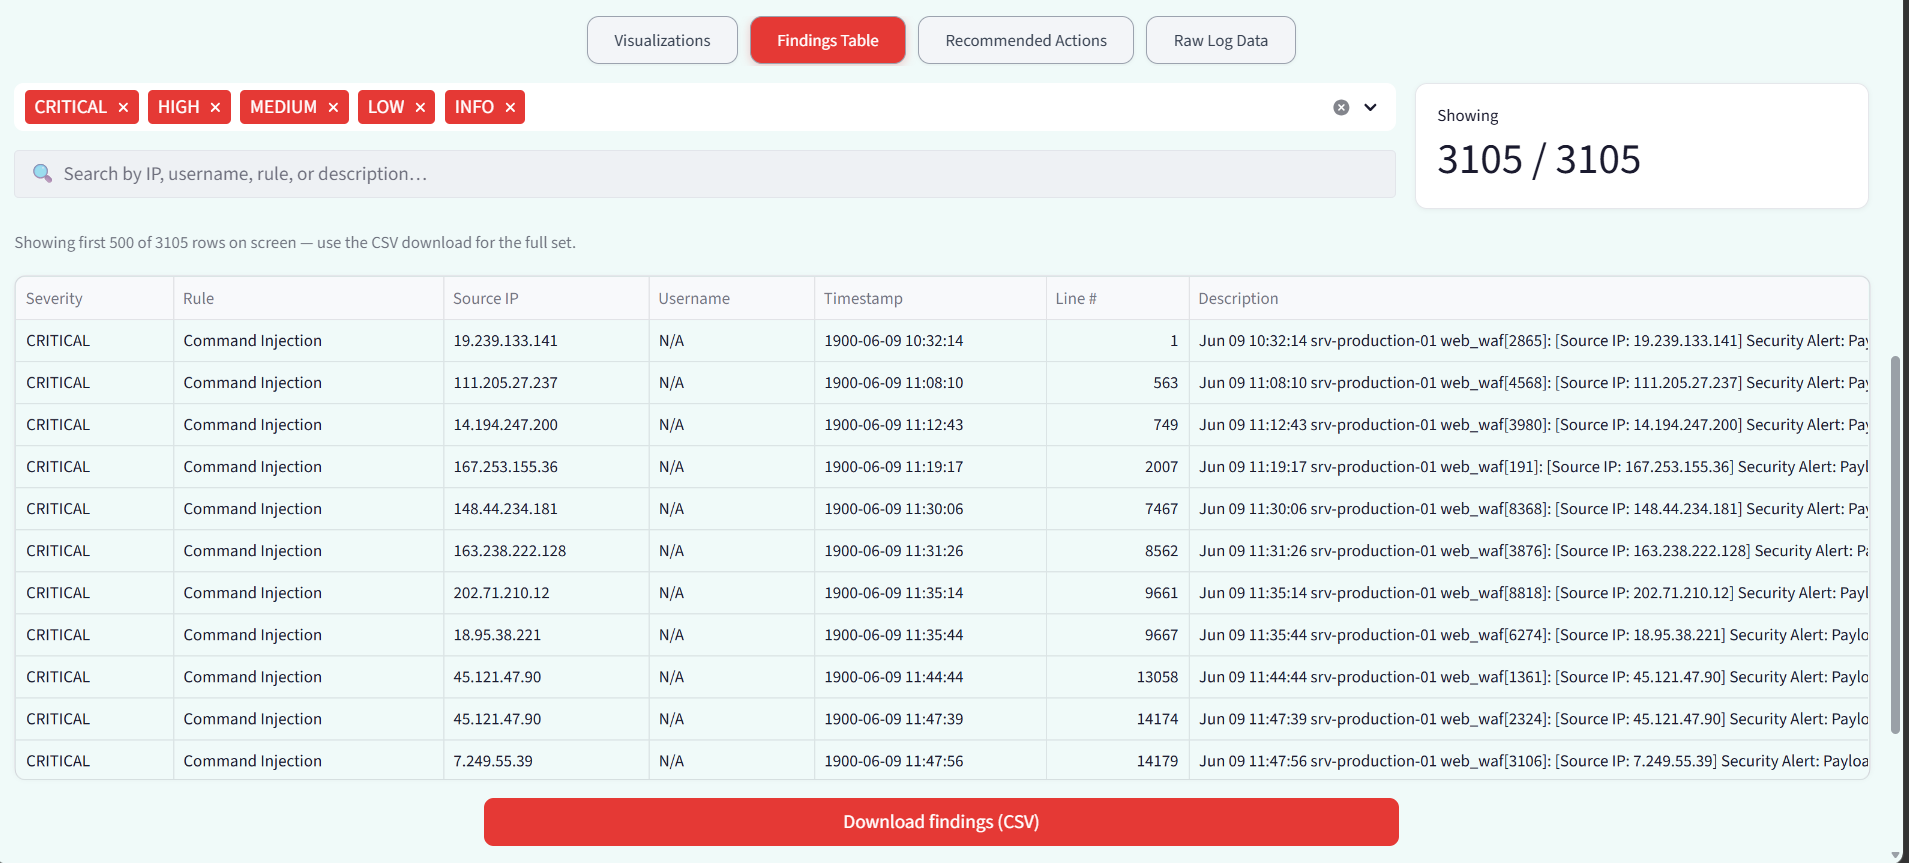
\includegraphics[width=0.92\textwidth]{findings.png}
\end{figure}

\subsubsection{Recommended Actions}
\begin{figure}[H]
    \centering
    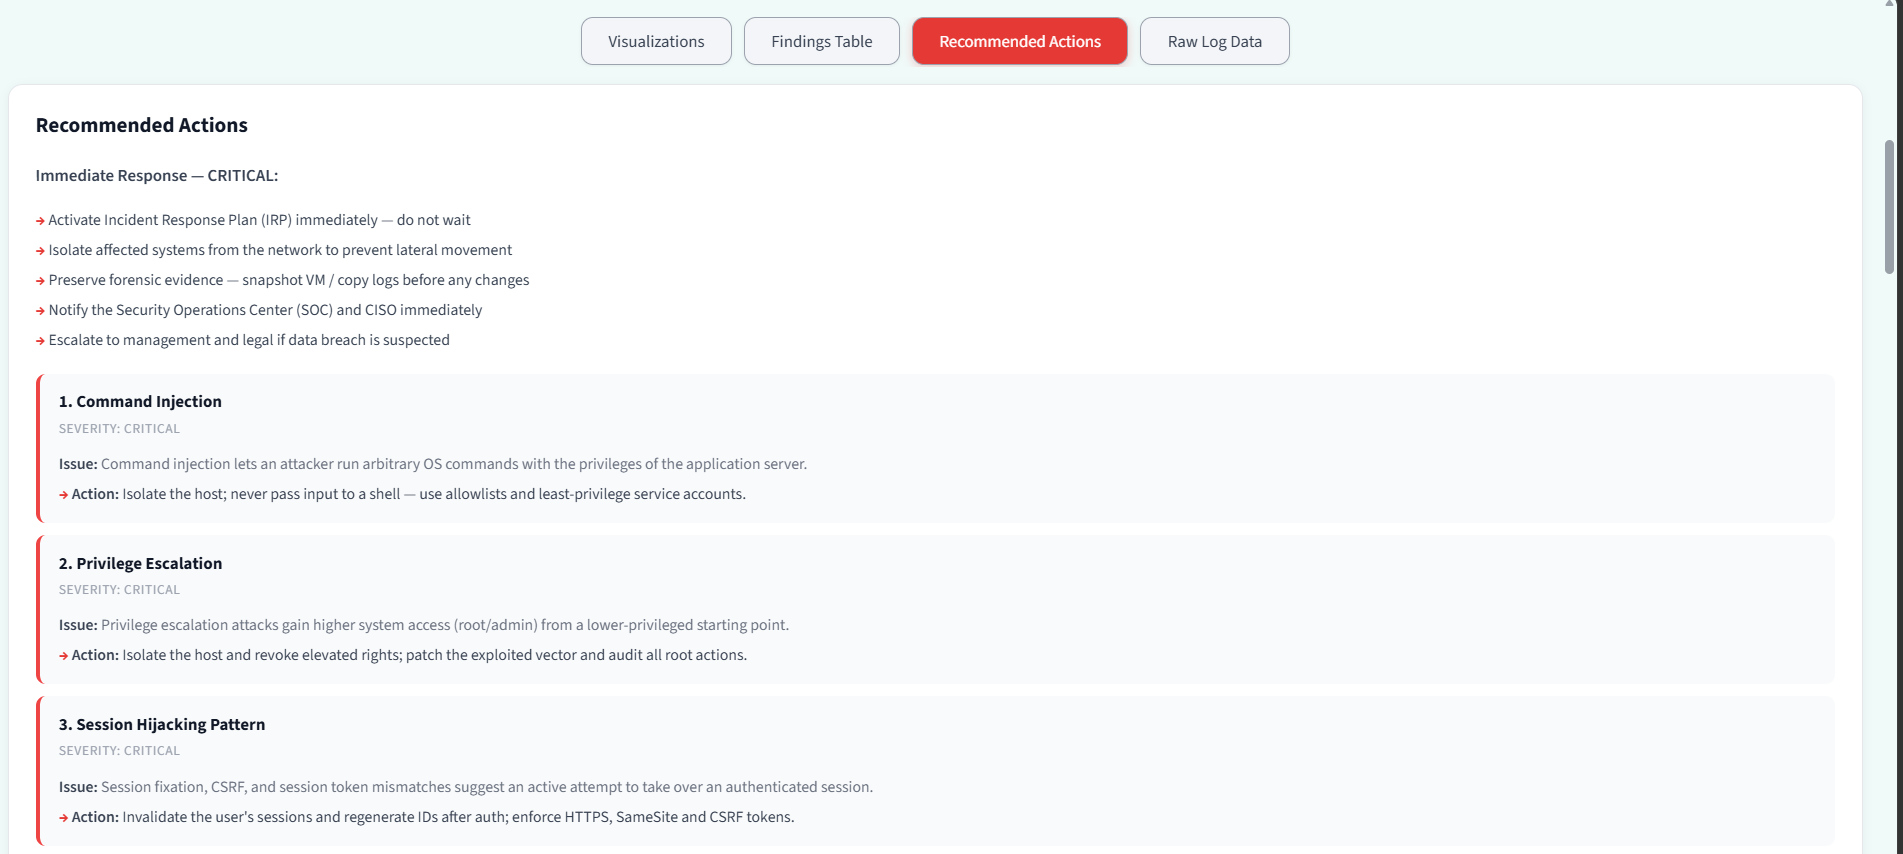
\includegraphics[width=0.92\textwidth]{recommended.png}
\end{figure}

\subsubsection{Raw Log Data}
\begin{figure}[H]
    \centering
    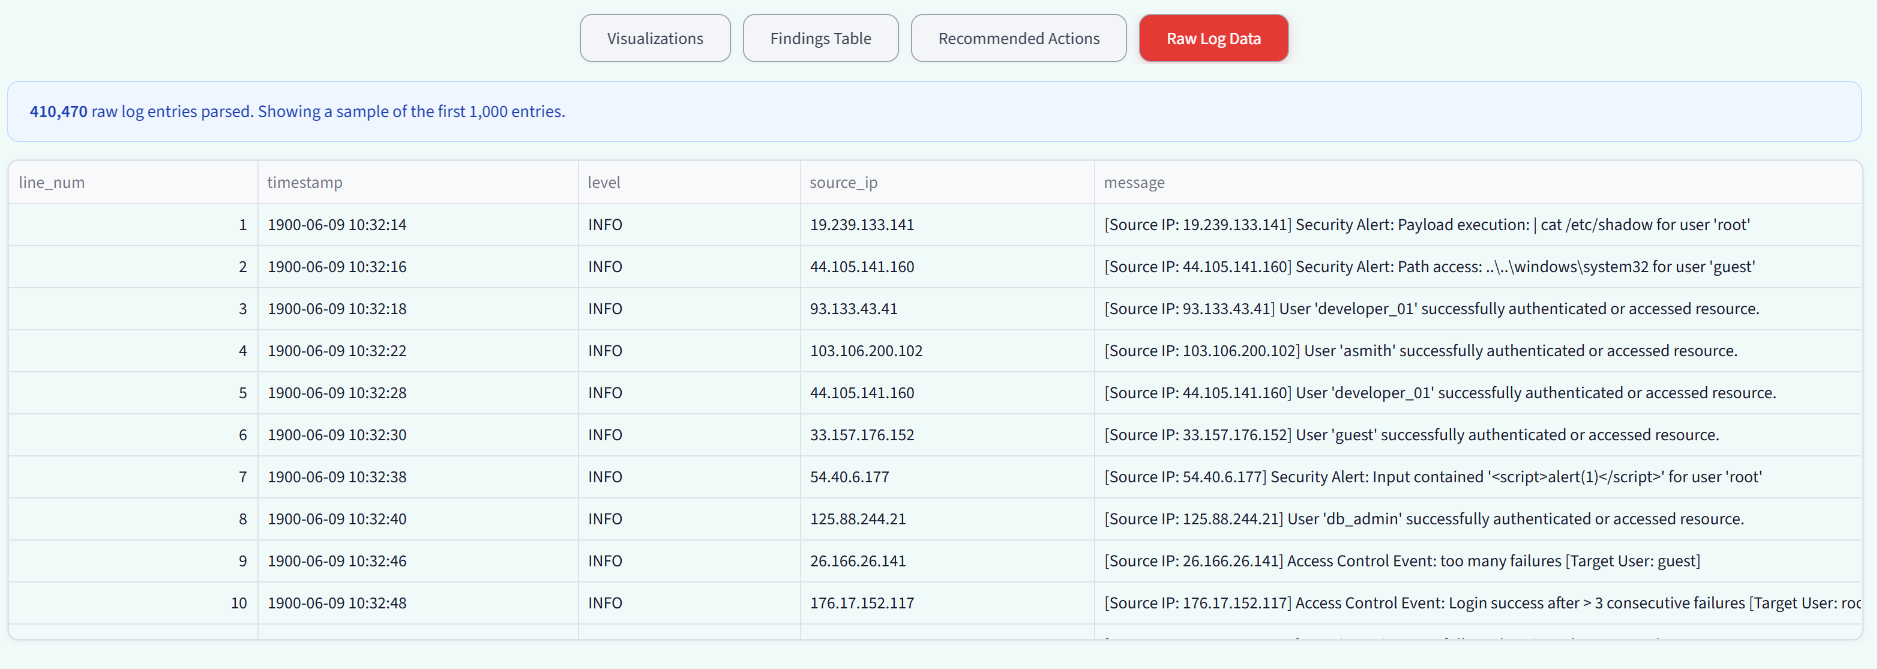
\includegraphics[width=0.92\textwidth]{raw_log.png}
\end{figure}

\section{Conclusion}
The Cybersecurity Log Intelligence System demonstrates that automated, enterprise-grade
security monitoring can be achieved without compromising data privacy or operational
resilience. By consolidating multi-file log analysis, framework-aligned threat detection,
role-based governance, and automated reporting into a single platform, the solution
directly addresses the inefficiencies and risks inherent in manual log review. The key
outcomes of the project are summarized below.
\begin{itemize}
    \item \textbf{Operational efficiency:} The system streamlines security operations by
          automating multi-file log analysis across 45 framework-aligned rules, reducing
          analyst workload and accelerating threat response.
    \item \textbf{Data governance and privacy:} On-demand reporting with no persistent
          storage of sensitive data ensures the solution meets stringent enterprise
          privacy and data-minimization requirements.
    \item \textbf{Enterprise-grade access control:} Role-based separation, Argon2id
          authentication, and enforced session policies uphold the principle of least
          privilege across all organizational stakeholders.
    \item \textbf{Scalability and business continuity:} Process-isolated workers with
          bounded concurrency and automatic fallback sustain performance under enterprise
          workloads while safeguarding service availability.
    \item \textbf{Compliance and audit readiness:} Standards-based rule mapping
          (MITRE ATT\&CK, OWASP, NIST, ISO 27001, CERT-In) and comprehensive audit
          logging position the system for regulatory compliance and security assurance.
    \item \textbf{Actionable intelligence:} Interactive dashboards, severity-ranked
          findings, and concise recommended actions translate raw log data into clear,
          decision-ready insights for security teams.
\end{itemize}
In conclusion, the platform delivers a scalable, and compliance-ready foundation
for enterprise log intelligence. Its privacy-first architecture and consistent enforcement
of role boundaries make it well-suited for modern organizational deployment. Future
enhancements may include integration with external SIEM platforms, real-time streaming
log ingestion, and machine-learning-based anomaly detection to further strengthen its
threat-identification capabilities.


\end{document}
